\documentclass{report}
\usepackage{amsmath,amssymb,graphicx,float,geometry,color}
\geometry{a4paper,total={170mm,257mm},left=20mm,top=20mm}

\title{\bf HKDSE MATH M2 Past Paper By Topic}
\author{STsAiR}
\date{\today}
\begin{document}
\maketitle
\tableofcontents
\chapter{Mathematical Induction}
\begin{enumerate}
	\item \textbf{HKDSE Math M2 Practice Paper Q3}\\
	Prove by mathematical induction that $4^n+15n - 1$ is divisible by 9 for all positive integers $n$. \\(5 marks)

	\item \textbf{HKDSE Math M2 2012 Q3}\\
	Prove, by mathematical induction, that for all positive integers $n$,$$\displaystyle 1 \times 2 + 2 \times 5 + 3 \times 8 + \cdots + n(3n-1) = n^2(n+1).$$ \\(5 marks)

	\item \textbf{HKDSE Math M2 2013 Q3}\\
	Prove, by mathematical induction, that for all positive integers $n$, $$\displaystyle 1 + \frac{1}{1 \times 4} + \frac{1}{4 \times 7} + \frac{1}{7 \times 10} + \cdots + \frac{1}{(3n-2)(3n+1)} = \frac{4n+1}{3n+1}.$$ \\(5 marks)

	\item \textbf{HKDSE Math M2 2015 Q8}
	\begin{enumerate}
		\item [(a)]Using mathematical induction, prove that $$\sin{\displaystyle\frac{x}{2}} \displaystyle\sum_{k = 1}^{n}\cos{kx} = \sin{\displaystyle\frac{nx}{2}}\cos{\displaystyle\frac{(n+1)x}{2}}$$ for all positive integers $n$.
		\item [(b)]Using (a), evaluate $\displaystyle\sum_{k = 1}^{567}\cos{\displaystyle\frac{k\pi}{7}}$.
	\end{enumerate}
	(8 marks)

	\item \textbf{HKDSE Math M2 2016 Q5}
	\begin{enumerate}
		\item [(a)]Using mathematical induction, prove that $$\displaystyle\sum_{k=1}^{n} (-1)^k k^2 = \frac{(-1)^n n(n+1)}{2}$$ for all positive integers $n$. 
		\item [(b)]Using (a), evaluate $\displaystyle\sum_{k=3}^{333} (-1)^{k+1} k^2$.
	\end{enumerate}
	(6 marks)

	\newpage

	\item \textbf{HKDSE Math M2 2018 Q6}
	\begin{enumerate}
		\item [(a)]Using mathematical induction, prove that $$\displaystyle \sum_{k = 1}^{n} k(k+4) = \frac{n(n+1)(2n+13)}{6}$$ for all positive integers $n$.
		\item [(b)] Using (a), evaluate $\displaystyle \sum_{k = 333}^{555} \left(\frac{k}{112}\right)\left(\frac{k+4}{223}\right)$.
	\end{enumerate}
	(7 marks)

	\item\textbf{HKDSE Math M2 2019 Q5}
	\begin{enumerate}
		\item [(a)] Using mathematical induction, prove that $$\displaystyle \sum_{k = n}^{2n} \frac{1}{k(k+1)} = \frac{(n+1)}{n(2n+1)}$$ for all positive integers $n$.
		\item [(b)] Using (a), evaluate $\displaystyle \sum_{k = 50}^{200} \frac{1}{k(k+1)}$.
	\end{enumerate}
	(7 marks)

	\item \textbf{HKDSE Math M2 2020 Q5}
	\begin{enumerate}
		\item [(a)]Using mathematical induction, prove that $$\displaystyle \sum_{k = 1}^{n} \frac{1}{k(k+1)(k+2)} = \frac{n(n+3)}{4(n+1)(n+2)}$$ for all positive integers $n$.
		\item [(b)] Using (a), evaluate $\displaystyle \sum_{k = 4}^{123} \frac{50}{k(k+1)(k+2)}$.
	\end{enumerate}
	(7 marks)

	\item \textbf{HKDSE Math M2 2021 Q2}\\
	Using mathematical induction, prove that $\displaystyle \sum_{k = 1}^{n} (3k^{5} + k^{3}) = \frac{n^{3} (n+1)^{3}}{2}$ for all positive integers $n$. \\
	(5 marks)

	\item \textbf{HKDSE Math M2 2022 Q3}
	\begin{enumerate}
		\item [(a)]Using mathematical induction, prove that $\displaystyle \sum_{k = 1}^{2n} (-1)^k k^2 = n(2n+1)$ for all positive integers $n$.
		\item [(b)] Using (a), evaluate $\displaystyle \sum_{k = 11}^{100} (-1)^k k^2$. 
	\end{enumerate}
	(7 marks)

	\item \textbf{HKDSE Math M2 2023 Q8}
	\begin{enumerate}
		\item [(a)]Let $\theta \in \mathbb{R}$. Using mathematical induction, prove that $\displaystyle \sin{\theta}\sum_{k=1}^{n}\sin{2k\theta} = \sin{n\theta}\sin{(n+1)\theta}$ for all positive integers $n$.
		\item [(b)] Using (a), find a pair of rational numbers $a$ and $b$ such that $\displaystyle\sum_{k = 1}^{111}\sin{\dfrac{k\pi}{11}}\cos{\dfrac{k\pi}{11}} = a\sin{b\pi}$, where $0 < b < \dfrac{1}{2}$.
	\end{enumerate}
	(8 marks)

\end{enumerate}

\chapter{Binomial Theorem}
\begin{enumerate}
	\item \textbf{HKDSE Math M2 Practice Paper Q1}\\
	Find the coefficient of $x^5$ in the expansion of $(2-x)^9$. \\(4 marks)

	\item \textbf{HKDSE Math M2 2012 Q2}\\
	It is given that 
	$$(1+ax)^n = 1 + 6x + 16x^2 +\text{terms involving higher powers of }x,$$
	where $n$ is a positive integer and $a$ is a constant. Find the values of $a$ and $n$.\\(5 marks)

	\item \textbf{HKDSE Math M2 2013 Q2}\\
	Suppose the coefficient of $x$ and $x^2$ in the expansion of $(1+ax)^n$ are $-20$ and 180 respectively. \\
	Find the values of $a$ and $n$. \\(4 marks)

	\item \textbf{HKDSE Math M2 2014 Q1}\\
	In the expansion of $(1-4x)^2(1+x)^n$, the coefficient of $x$ is 1.
	\begin{enumerate}
		\item [(a)]Find the value of $n$. 
		\item [(b)]Find the coefficient of $x^2$. 
	\end{enumerate}
	(4 marks)

	\item \textbf{HKDSE Math M2 2016 Q1}\\
	Expand $(5+x)^4$. \\Hence, find the constant term in the expansion of $(5+x)^4\left(1-\displaystyle\frac{2}{x}\right)^3$. \\(5 marks)

	\item \textbf{HKDSE Math M2 2017 Q2}\\
	Let $\displaystyle(1+ax)^8 = \sum_{k = 0}^{8} \lambda _{k} x^{k}$ and $\displaystyle(b+x)^9 = \sum_{k = 0}^{9} \mu _{k} x^{k}$, where $a$ and $b$ are constants. \\
	It is given that $\lambda_2 : \mu_7 = 7:4$ and $\lambda_1 + \mu_8  + 6 = 0$. Find $a$.  \\(5 marks)

	\item  \textbf{HKDSE Math M2 2018 Q2}\\
	Expand $(x+3)^5$. Hence, find the coefficient of $x^3$ in the expansion of $(x+3)^5 \displaystyle\left(x - \frac{4}{x}\right) ^ 2$. \\(5 marks)

	\newpage

	\item \textbf{HKDSE Math M2 2019 Q2}\\
	Let $P(x) = \begin{vmatrix}
		x+\lambda & 1 & 2  \\ 
		0 & (x+\lambda)^2 & 3 \\ 
		4 & 5 & (x+\lambda)^3  \notag
		\end{vmatrix}$, where $\lambda \in \mathbb{R}$. \\
	It is given that the coefficient of $x^3$ in the expansion of $P(x)$ is 160. Find
	\begin{enumerate}
		\item $\lambda$,
		\item $P'(0)$. 
	\end{enumerate}
	(5 marks)

	\item \textbf{HKDSE Math M2 2020 Q1}
	\begin{enumerate}
		\item [(a)] Expand $(1-x)^4$.
		\item [(b)] Find the constant $k$ such that the coefficient of $x^2$ in the expansion of $(1+kx)^9(1-x)^4$ is $-3$.
	\end{enumerate}
	(4 marks)

	\item \textbf{HKDSE Math M2 2021 Q3}\\
	The coefficient of $x^2$ in the expansion of $(1-4x)^n$ is 240, where $n$ is a positive integer. Find
	\begin{enumerate}
		\item[(a)]
		$n$,
		\item[(b)]
		the coefficient of $x^4$ in the expansion of $\displaystyle(1-4x)^n\left(1+\frac{2}{x}\right)^5$. 
	\end{enumerate}
	(6 marks)
	
	\item \textbf{HKDSE Math M2 2022 Q5}\\
	Let $n$ be an integer greater than 1. Define $\displaystyle (a+x)^n  = \sum_{k = 0}^{n} \mu_k x^k$, where $a$ is a constant. \\
	It is given that $\mu_2 = -10$.
	\begin{enumerate}
		\item [(a)] Explain why $a$ is a negative number and $n$ is an odd number. 
		\item [(b)] Let $\displaystyle (bx-1)^n  = \sum_{k = 0}^{n} \lambda_k x^k$, where $b$ is a constant. If $\lambda_0 = \mu_0$ and $\lambda_1 = 2\mu_1$, find $a$, $b$ and $n$.
	\end{enumerate}
	(6 marks)

	\item \textbf{HKDSE Math M2 2023 Q1}\\
	Let $a$ be a constant. If the coefficient of $x$ in the expansion of $(2-3x)^5\left(x + \dfrac{a}{x}\right)^2$ is $\dfrac{160}{3}$, find $a$ and the coefficient of $x^2$ in the expansion.\\
	(5 marks)

\end{enumerate}

\chapter{Trigonometry}
\begin{enumerate}
	\item \textbf{HKDSE Math M2 Sample Paper Q5}\\
	By considering $\displaystyle\sin{\frac{\pi}{7}}\cos{\frac{\pi}{7}}\cos{\frac{2\pi}{7}}\cos{\frac{3\pi}{7}}$, find the value of $\displaystyle\cos{\frac{\pi}{7}}\cos{\frac{2\pi}{7}}\cos{\frac{3\pi}{7}}$. \\(4 marks)

	\item \textbf{HKDSE Math M2 Sample Paper Q10}\\
	Let $0^{\circ} < \theta < 180^{\circ}$ and define $A = \begin{pmatrix}\cos{\theta}&-\sin{\theta}\\\sin{\theta}&\cos{\theta}\\\end{pmatrix}$. 
	\begin{enumerate}
		\item [(a)]Prove, by mathematical induction, that
		$$A^n = \begin{pmatrix}\cos{n\theta}&-\sin{n\theta}\\\sin{n\theta}&\cos{n\theta}\\\end{pmatrix}$$ for all positive integers $n$.
		\item [(b)]Solve $\sin{3\theta} + \sin{2\theta} + \sin{\theta} = 0$.
		\item [(c)]It is given that $A^3 + A^2 + A = \begin{pmatrix}a&0\\0&a\\\end{pmatrix}$.\\Find the value(s) of $a$. 
	\end{enumerate}
	(8 marks)

	\item \textbf{HKDSE Math M2 Practice Paper Q4}
	\begin{enumerate}
		\item [(a)]Let $x = \tan{\theta}$, show that $$\displaystyle\frac{2x}{1+x^2} = \sin{2\theta}.$$ 
		\item [(b)]Using (a), find the greatest value of $\displaystyle\frac{(1+x)^2}{1+x^2}$, where $x$ is real.
	\end{enumerate}
	(5 marks)

	\newpage

	\item \textbf{HKDSE Math M2 Practice Paper Q13}
	\begin{enumerate}
		\item[(a)]Let $f(x)$ be an odd function for $-p \leq x \leq p$, where $p$ is a positive constant.
		Prove that $$\displaystyle\int_0^{2p} f(x-p)\,dx = 0.$$
		Hence evaluate $\displaystyle\int_0^{2p} [f(x-p)+q]\,dx $, where $q$ is a constant. \\(4 marks)
		\item[(b)]Prove that $$\displaystyle\frac{\sqrt{3} + \tan{\left(x - \displaystyle\frac{\pi}{6}\right)}}{\sqrt{3} - \tan{\left(x - \displaystyle\frac{\pi}{6}\right)}} = \frac{1+\sqrt{3}\tan{x}}{2}.$$ \\(2 marks)
		\item[(c)]Using (a) and (b), or otherwise, evaluate $\displaystyle\int_0^{\tfrac{\pi}{3}} \ln{(1 + \sqrt{3}\tan{x})} \,dx$. \\(4 marks)
	\end{enumerate}

	\item \textbf{HKDSE Math M2 2012 Q10}\\
	In Figure 5, $OAB$ is an isosceles triangle with $OA = OB$, $AB = 1$, $AY = y$, $\angle AOY = \theta$ and $\angle BOY = 3\theta$. 
	\begin{figure}[H]
		\centering
		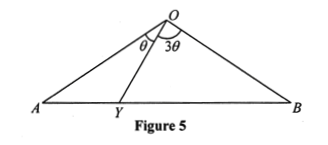
\includegraphics[width = .5\linewidth]{2012Figure5}
	\end{figure}
	\begin{enumerate}
		\item [(a)]Show that $y = \displaystyle\frac{1}{4}\sec^2{\theta}$.
		\item [(b)]Find the range of values of $y$. 
		
		[Hint: you may use the identity $\sin{3\theta} = 3\sin{\theta} - 4\sin^3{\theta}$.]
	\end{enumerate}
	(6 marks)

	\newpage

	\item \textbf{HKDSE Math M2 2012 Q13}
	\begin{enumerate}
		\item [(a)]
		\begin{enumerate}
			\item [(i)]Suppose $\tan{u} = \displaystyle\frac{-1 + \cos{\displaystyle\frac{2\pi}{5}}}{\sin{\displaystyle\frac{2\pi}{5}}}$, where $\displaystyle\frac{-\pi}{2} < u < \frac{\pi}{2}$. \\
			Show that $u = \displaystyle\frac{-\pi}{5}$. 
			\item [(ii)]Suppose $\tan{v} = \displaystyle\frac{1+\cos{\displaystyle\frac{2\pi}{5}}}{\sin{\displaystyle\frac{2\pi}{5}}}$. \\
			Find $v$, where $\displaystyle\frac{-\pi}{2} < v < \frac{\pi}{2}$.
		\end{enumerate}
		(4 marks)
		\item[(b)]
		\begin{enumerate}
			\item[(i)]Express $x^2 + 2x\cos{\displaystyle\frac{2\pi}{5}} + 1$ in the form $(x+a)^2 + b^2$, where $a$ and $b$ are constants. 
			\item[(ii)]Evaluate $\displaystyle\int_{-1}^{1}\frac{\sin{\displaystyle\frac{2\pi}{5}}}{x^2 + 2x\cos{\displaystyle\frac{2\pi}{5}}+1}\, dx$.
		\end{enumerate}
		(6 marks)
		\item[(c)]Evaluate $\displaystyle\int_{-1}^{1}\frac{\sin{\displaystyle\frac{7\pi}{5}}}{x^2 + 2x\cos{\displaystyle\frac{7\pi}{5}}+1} \,dx$. \\(3marks)
	\end{enumerate}

	\item \textbf{HKDSE Math M2 2013 Q7}
	\begin{enumerate}
		\item [(a)]Prove the identity $\tan{x} = \displaystyle\frac{\sin{2x}}{1+\cos{2x}}$. 
		\item [(b)]Using (a), prove the identity $$\tan{y} = \displaystyle\frac{\sin{8y}\cos{4y}\cos{2y}}{(1+\cos{8y})(1+\cos{4y})(1+\cos{2y})}.$$
	\end{enumerate}
	(5 marks)

	\newpage

	\item \textbf{HKDSE Math M2 2014 Q13}
	\begin{enumerate}
		\item [(a)]Prove that $$1 - \cos{4\theta} - 2\cos{2\theta}\sin^2{2\theta} = 16\cos^2{\theta}\sin^4{\theta}.$$ \\(2 marks)
		\item [(b)]Show that $\displaystyle\int_{0}^{n\pi} \cos^2{x}\sin^4{x} \,dx = \displaystyle\frac{n\pi}{16}$, where $n$ is a positive integer.\\(4 marks)
		\item [(c)]Let $f(x)$ be a continuous function such that $f(k-x) = f(x)$, where $k$ is a constant. Show that $$\displaystyle\int_{0}^k xf(x)\, dx = \frac{k}{2} \int_{0}^k f(x) \,dx.$$
		(4 marks)
		\item [(d)]Figure 5 shows the shaded region bounded by curve $y = cos^2{x} \sin^4{x}$ and the $x$-axis, \\
		where $\pi \leq x \leq 2\pi$. Find the volume of the solid of revolution when the shaded region is revolved about the $y$-axis.\\
		(4 marks)
			\begin{figure}[H]
				\centering
				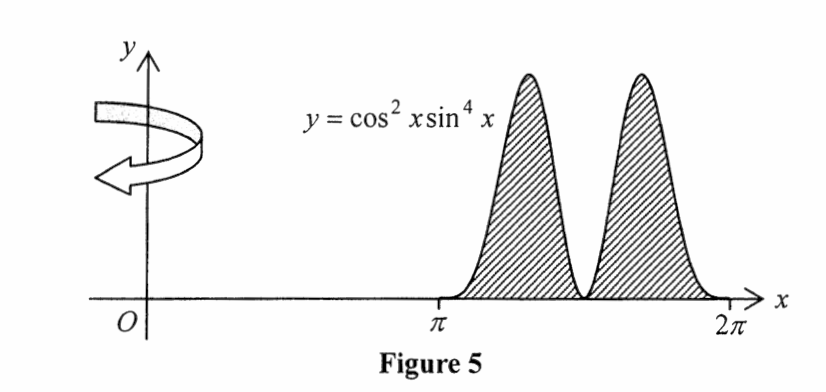
\includegraphics[width = .5\linewidth]{2014Figure5}
			\end{figure}
	\end{enumerate}

	\item \textbf{HKDSE Math M2 2015 Q7}
	\begin{enumerate}
		\item [(a)]Prove that $$\sin^2{x}\cos^2{x} = \displaystyle\frac{1 - \cos{4x}}{8}.$$ 
		\item [(b)]Let $f(x) = \sin^4{x} + \cos^4{x}$. 
		\begin{enumerate}
			\item [(i)]Express $f(x)$ in the form $A\cos{Bx} + C$, where $A$, $B$ and $C$ are constants.
			\item [(ii)]Solve the equation $8f(x) = 7$, where $ 0\leq  x \leq \displaystyle\frac{\pi}{2}$.
		\end{enumerate}
	\end{enumerate}
	(7 marks)

	\item \textbf{HKDSE Math M2 2016 Q6}
	\begin{enumerate}
		\item [(a)]Prove that $x+1$ is a factor of $4x^3+2x^2-3x-1$. 
		\item [(b)]Express $\cos{3\theta}$ in terms of $\cos{\theta}$.
		\item [(C)]Using the results of (a) and (b), prove that $$\cos{\displaystyle\frac{3\pi}{5}} = \displaystyle\frac{1-\sqrt{5}}{4}.$$
	\end{enumerate}
	(6 marks)

	\newpage

	\item\textbf{HKDSE Math M2 2017 Q7}
	\begin{enumerate}
		\item[(a)]Prove that $\sin{3x} = 3\sin{x}  - 4\sin^3{x}$. 
		\item[(b)]Let $\displaystyle\frac{\pi}{4} < x < \frac{\pi}{2}$.
		\begin{enumerate}
			\item [(i)]Prove that $$\displaystyle\frac{\sin{3\left(x - \displaystyle\frac{\pi}{4}\right)}}{\sin{\left(x - \displaystyle\frac{\pi}{4}\right)}} = \frac{\cos{3x} + \sin{3x}}{\cos{x} - \sin{x}}.$$
			\item [(ii)]Solve the equation $\displaystyle\frac{\cos{3x} + \sin{3x}}{\cos{x} - \sin{x}} = 2$.
		\end{enumerate}
	\end{enumerate}
	(8 marks)

	\item \textbf{HKDSE Math M2 2018 Q3}
	\begin{enumerate}
		\item [(a)] If $\cot{A} = 3\cot{B}$, prove that $\sin{(A+B)} = 2\sin{(B-A)}$. 
		\item [(b)] Using (a), solve the equation $\displaystyle\cot{(x+\frac{4\pi}{9})} = 3\cot{(x+\frac{5\pi}{18})}$, where $0 \leq x \leq \displaystyle\frac{\pi}{2}$.
	\end{enumerate}
	(5 marks)

	\item \textbf{HKDSE Math M2 2019 Q10}
	\begin{enumerate}
		\item [(a)] Let $0 \leq x \leq \displaystyle\frac{\pi}{4}$. Prove that $\displaystyle\frac{1}{2+\cos{2x}} = \frac{\sec^2{x}}{2+\sec^2{x}}$. \\(1 mark) 
		\item [(b)] Evaluate $\displaystyle \int_{0}^{ \tfrac{\pi}{4}} \frac{1}{2+\cos{2x}}\,dx$. \\(3 marks)
		\item [(c)] Let $f(x)$ be a continuous function defined on $\mathbb{R}$ such that $f(-x) = -f(x)$ for all $x \in \mathbb{R}$. Prove that $$\displaystyle\int_{-a}^{a} f(x)\ln{(1+e^x)}\,dx = \int_{0}^{a} xf(x)\,dx$$ for any $a \in \mathbb{R}  $. \\(4 marks)
		\item [(d)] Evaluate $\displaystyle \int_{\tfrac{-\pi}{4}}^{\tfrac{\pi}{4}}  \frac{\sin{2x}}{(2+\cos{2x})^2}\ln(1 + e^x)\,dx$. \\(5 marks)
	\end{enumerate}
	\item \textbf{HKDSE Math M2 2020 Q3}
	\begin{enumerate}
		\item [(a)] Let $x$ be an angle which is not a multiple of $30^\circ$. Prove that 
		\begin{enumerate}
			\item [(i)]$\tan{3x} = \displaystyle \frac{3\tan{x} - \tan^3{x}}{1-3\tan^2{x}}$, 
			\item [(ii)] $\tan{x} \tan(60^\circ - x)\tan(60^\circ + x) = \tan{3x}$. 
		\end{enumerate}
		\item [(b)] Using (a)(ii), prove that $\tan{55^\circ}\tan{65^\circ}\tan{75^\circ} = \tan{85^\circ}$.
	\end{enumerate}
	(6 marks)

	\newpage

	\item \textbf{HKDSE Math M2 2020 Q10}
	\begin{enumerate}
		\item [(a)]Using integration by substitution, prove that $$\displaystyle \int_{\tfrac{\pi}{12}}^{\tfrac{\pi}{6}}  \ln{\left(\sin{\left(\frac{\pi}{4} - x\right)}\right)}\,dx = \int_{\tfrac{\pi}{12}}^{\tfrac{\pi}{6}}  \ln{(\sin{x})}\,dx.$$ \\(3 marks)
		\item [(b)] Using (a), evaluate $\displaystyle \int_{\tfrac{\pi}{12}}^{\tfrac{\pi}{6}}  \ln{(\cot{x} - 1)}\,dx$. \\(3 marks)
		\item [(c)] 
		\begin{enumerate}
			\item [(i)] Using $\cot{(A-B)} = \displaystyle \frac{\cot{A}\cot{B}+1}{\cot{B} - \cot{A}}$, or otherwise, prove that $\displaystyle \cot{\frac{\pi}{12}} = 2 + \sqrt{3}$. 
			\item [(ii)] Using integration by parts, prove that $$\displaystyle\int_{\tfrac{\pi}{12}}^{\tfrac{\pi}{6}}  \frac{x\csc^2{x}}{\cot{x} -1}\,dx = \frac{\pi}{8} \ln{(2 + \sqrt{3})}.$$
		\end{enumerate}
	    (7 marks)
	\end{enumerate}

	\item \textbf{HKDSE Math M2 2021 Q4}
	\begin{enumerate}
		\item [(a)] Prove that $\cos{2x} + \cos {4x} + \cos {6x} = 4\cos{x}\cos{2x}\cos{3x} -1$.
		\item [(b)] Solve the equation $\cos{4\theta} + \cos{8\theta} + \cos{12\theta} = -1$, where $\displaystyle0 \leq \theta \leq \frac{\pi}{2}$.
	\end{enumerate}
	(6 marks)

	\item \textbf{HKDSE Math M2 2022 Q2}\\
	Let $\displaystyle \frac{\pi}{4} < \theta < \frac{\pi}{2}$.
	\begin{enumerate}
		\item [(a)] Prove that $\displaystyle \frac{\tan{\theta}}{1-\cot{\theta}} + \frac{\cot{\theta}}{1-\tan{\theta}} = 1+\sec{\theta}\csc{\theta}$.
		\item [(b)] Solve the equation $\displaystyle \frac{\tan{\theta}}{1-\cot{\theta}} + \frac{\cot{\theta}}{1-\tan{\theta}} = 5$.
	\end{enumerate}
	(5 marks)

	\item \textbf{HKDSE Math M2 2023 Q4}
	\begin{enumerate}
		\item[(a)]Prove that $\cos{3x} = 4\cos^3{x} - 3\cos{x}$.
		\item[(b)]Using (a), solve the equation $\sec^3{x} - 6\sec^2{x} + 8 = 0$, where $\dfrac{\pi}{2} < x < \dfrac{3\pi}{2}$.
	\end{enumerate}
	(5 marks)

	\item \textbf{HKDSE Math M2 2023 Q8}
	\begin{enumerate}
		\item [(a)]Let $\theta \in \mathbb{R}$. Using mathematical induction, prove that $\displaystyle \sin{\theta}\sum_{k=1}^{n}\sin{2k\theta} = \sin{n\theta}\sin{(n+1)\theta}$ for all positive integers $n$.
		\item [(b)] Using (a), find a pair of rational numbers $a$ and $b$ such that $\displaystyle\sum_{k = 1}^{111}\sin{\dfrac{k\pi}{11}}\cos{\dfrac{k\pi}{11}} = a\sin{b\pi}$, where $0 < b < \dfrac{1}{2}$.
	\end{enumerate}
	(8 marks)

\end{enumerate}

\chapter{Definition of Differentiation(First Principles)}
\begin{enumerate}
	\item \textbf{HKDSE Math M2 Sample Paper Q1}\\
	Find $\displaystyle\frac{d}{dx}(\sqrt{2x})$ from first principles. \\(4 marks)

	\item \textbf{HKDSE Math M2 Practice Paper Q6}\\
	Find $\displaystyle\frac{d}{dx}\left(\frac{1}{x}\right)$ from first principles. \\(4 marks)	

	\item \textbf{HKDSE Math M2 2012 Q1}\\
	Let $f(x) = e^{2x}$. Find $f'(0)$ from first principles. \\(3 marks)	

	\item \textbf{HKDSE Math M2 2013 Q1}\\
	Find $\displaystyle\frac{d}{dx} (\sin{2x})$ from first principles. \\(4 marks)	

	\item \textbf{HKDSE Math M2 2014 Q2}\\
	Consider the curve $C : y = x^3-3x$. 
	\begin{enumerate}
		\item [(a)]Find $\displaystyle\frac{dy}{dx}$ from  first principles. 
		\item [(b)]Find the range of $x$ where $C$ is decreasing.
	\end{enumerate}
	(5 marks)

	\item \textbf{HKDSE Math M2 2015 Q1}\\
	Find $\displaystyle \frac{d}{dx} (x^5+4)$ from first principles. \\(4 marks)

	\item \textbf{HKDSE Math M2 2016 Q2}\\
	Prove that $\displaystyle\frac{1}{\sqrt{x}} - \frac{1}{\sqrt{x+h}} = \frac{h}{(x+h)\sqrt{x} + x\sqrt{x+h}}$. Hence, find $\displaystyle \frac{d}{dx} \sqrt{\displaystyle\frac{3}{x}}$ from first principles. \\(5 marks)

	\item \textbf{HKDSE Math M2 2017 Q1}\\
	Let $\displaystyle \frac{d}{d\theta} \sec{6\theta}$ from first principles. \\(5 marks)	

	\item \textbf{HKDSE Math M2 2018 Q1}\\
	Let $\displaystyle f(x) = (x^2-1)e^x$.  Express $f(1+h)$ in terms of $h$. Hence, find  $f'(1)$ from first principles. \\(4 marks)

    \newpage

	\item \textbf{HKDSE Math M2 2019 Q1}\\
	Let $\displaystyle f(x) = \frac{10x}{7+3x^2}$. Prove that $f(1+h) - f(1) = \displaystyle\frac{4h-3h^2}{10+6h+3h^2}$. Hence, find  $f'(1)$ from first principles. \\(4 marks)

	\item \textbf{HKDSE Math M2 2020 Q2}\\
	Define $\displaystyle f(x) = \frac{x}{\sqrt{2+x}}$, for all $x > -2$. Find $f'(2)$ from first principles. \\(4 marks)

	\item \textbf{HKDSE Math M2 2021 Q1}\\
	Let $\displaystyle f(x) = \frac{1}{3x^{2}+4}$. Find $f'(x)$ from first principles. \\(4 marks)

	\item \textbf{HKDSE Math M2 2022 Q1}\\
	Let $\displaystyle g(x) = \frac{1}{\sqrt{5x+4}}$, where $x > 0$. Prove that $\displaystyle g(1+h)-g(1) = \frac{-5h}{3\sqrt{5h+9}(3+\sqrt{5h+9})}$. Hence, find $g'(1)$ from first principles. \\
	(4 marks)

	\item \textbf{HKDSE Math M2 2023 Q2}\\
	Let $f(x) = -x \sin{x}$.
	\begin{enumerate}
		\item [(a)]Prove that $f\left(\dfrac{\pi}{2} + h\right) - f\left(\dfrac{\pi}{2}\right) = \pi \sin^2{\left(\dfrac{h}{2}\right)} - h \cos{h}$.
		\item [(b)]Using (a), find $f'\left(\dfrac{\pi}{2}\right)$ from the first principles.
	\end{enumerate}
	(5 marks)

\end{enumerate}

\chapter{Applications of Differentiation}
\begin{enumerate}
	\item \textbf{HKDSE Math M2 Sample Paper Q2}\\
	A snowball in a shape of sphere is melting with its volume decreasing at a constant rate of 4 cm$^3$s$^{-1}$. \\
	When its radius is 5 cm, find the rate of change of its radius. \\(4 marks)

	\item \textbf{HKDSE Math M2 Sample Paper Q6}\\
	Let $C$ be the curve $3e^{x-y} = x^2+y^2+1$. \\
	Find the equation of the tangent to $C$ at the point $(1,1)$. \\(5 marks)

	\item \textbf{HKDSE Math M2 Sample Paper Q12}\\
	Let $\displaystyle f(x) = \frac{4}{x-1} - \frac{4}{x+1} -1$, where $x \neq \pm 1$.
	\begin{enumerate}
		\item [(a)]
		\begin{enumerate}
			\item [(i)]Find the $x$- and $y$-intercept(s) of the graph of $y = f(x)$. 
			\item [(ii)]Find $f'(x)$ and prove that 
			$$f''(x) = \displaystyle\frac{16(3x^2 + 1)}{(x-1)^3(x+1)^3}$$
			for $x \neq \pm 1$. 
			\item [(iii)]For the graph of $y = f(x)$, find all the extreme points and show that there are no points of inflexion.
		\end{enumerate}
		(6 marks)
		\item [(b)]Find all the asymptote(s) of the graph of $y = f(x)$. \\(2 marks)
		\item [(c)]Sketch the graph of $y = f(x)$. \\(3 marks)
		\item [(d)]Let $S$ be the area bounded by the graph of $y = f(x)$, the straight lines $x = 3$, $x = a $ $(a > 3)$ and $y = -1$. \\
		Find $S$ in terms of $a$. Deduce that $S < 4\ln{2}$. \\(3 marks)
  	\end{enumerate}
	
	\item \textbf{HKDSE Math M2 Practice Paper Q7}\\
	Let $f(x) = e^x(\sin{x} + \cos{x})$. 
	\begin{enumerate}
		\item[(a)]Find $f'(x)$ and $f''(x)$. 
		\item[(b)]Find the value of $x$ such that $f''(x) - f'(x) + f(x) = 0$ for $0 \leq x \leq \pi$.
	\end{enumerate}
	(5 marks)

	\item \textbf{HKDSE Math M2 Practice Paper Q9}\\
	Find the equations of the two tangents to the curve $x^2 - xy -2y^2 -1 =0$ which are parallel to the straight line $y = 2x+1$. \\(6 marks)

	\item \textbf{HKDSE Math M2 2012 Q5}\\
	Find the minimum point(s) and asymptote(s) of the graph of $\displaystyle y = \frac{x^2+x+1}{x+1}$. \\(6 marks)

	\newpage

	\item \textbf{HKDSE Math M2 2012 Q6}\\
	A frustum of height $H$ is made by cutting off a right circular cone of base radius $r$ from a right circular cone of base radius $R$ (See Figure 1). It is given that the volume of the frustum is $\displaystyle\frac{\pi}{3}H(r^2 + rR + R^2)$. \\
	An empty glass is in the form of an inverted frustum described above with height 10 cm, the radii of the rim and the base 4 cm and 3 cm respectively. Water is being poured into the glass. Let $h$ cm $(0 \leq h \leq 10)$ be the depth of the water inside the glass at time $t$ s (see Figure 2).
	\begin{figure}[H]
		\centering
		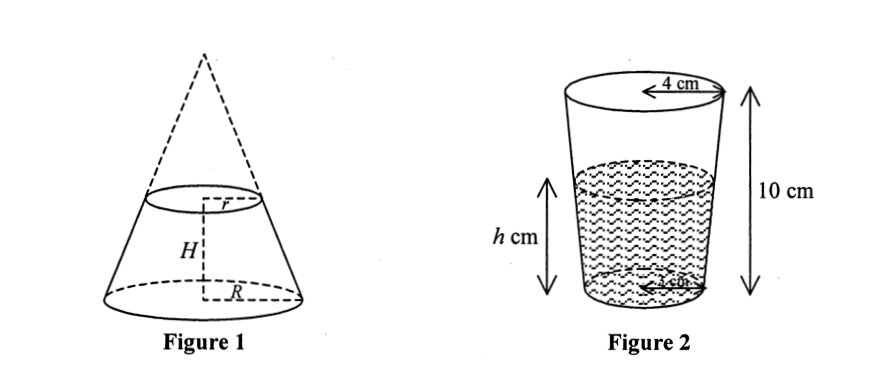
\includegraphics[width = .6\linewidth]{2012Figure1n2}
	\end{figure}
	\begin{enumerate}
		\item [(a)]Show that the volume $V$ cm$^{3}$ of water inside the glass at time $t$ s is given by 
		$$V = \displaystyle\frac{\pi}{300}(h^3+90h^2+2700h).$$
		\item [(b)]If the volume of water in the glass is increasing at the rate $7\pi$ cm$^3$ s$^{-1}$, find the rate of increase of depth of water at the instant when $h = 5$.
	\end{enumerate}
	(6 marks)

	\newpage

	\item \textbf{HKDSE Math M2 2012 Q14}\\
	Consider the curve $\Gamma : y = kx^p$, where $k>0$, $p > 0$. In Figure 7, the tangent to $\Gamma$ at $A(a, ka^{p})$ cuts the $x$-axis at $B(-a, 0)$, where $a>0$.
	\begin{figure}[H]
		\centering
		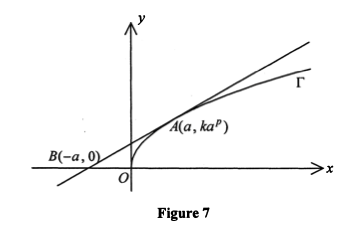
\includegraphics[width = .5\linewidth]{2012Figure7}
	\end{figure}
	\begin{enumerate}
		\item [(a)]Show that $\displaystyle p = \frac{1}{2}$. \\(3 marks)
		\item [(b)]Suppose that $a = 1$. As shown in Figure 8, the circle $C$, with radius 2 and centre on the $y$-axis, touches $\Gamma$ at point $A$.
		\begin{figure}[H]
			\centering
			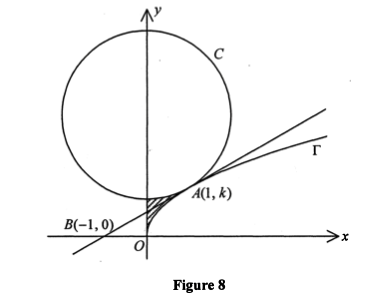
\includegraphics[width = .5\linewidth]{2012Figure8}
		\end{figure}
		\begin{enumerate}
			\item [(i)]Show that $\displaystyle k = \frac{2\sqrt{3}}{3}$. 
			\item [(ii)]Find the area of the shaded region bounded by $\Gamma$, $C$ and the $y$-axis.
		\end{enumerate}
		(9 marks)
	\end{enumerate}

	\item \textbf{HKDSE Math M2 2013 Q5}\\
	Consider a continuous function $f(x) = \displaystyle\frac{3 -3x^2}{3+x^2}$. It is given that $$\begin{array}{|c|c|c|c|c|c|c|c|}
		\hline
		x & x<-1 & -1 & -1<x<0 & 0 & 0<x<1 & 1 & x>1\\
		\hline
		f'(x) & + & + & + & 0 & - & - & -\\
		\hline		
		f''(x) & + & 0 & - & - & - & 0 & +\\
		\hline
    \end{array}$$
	(`$+$' and `$-$' denote `positive value' and `negative value' respectively.)
	\begin{enumerate}
		\item [(a)]Find all the maximum and/or minimum point(s) and point(s) of inflexion.
		\item [(b)]Find the asymptote(s) of the graph of $y = f(x)$. 
		\item [(c)]Sketch the graph of $y = f(x)$.
	\end{enumerate}
	(6 marks)

	\newpage

	\item \textbf{HKDSE Math M2 2013 Q12}\\
	In Figure 3, the distance between two houses $A$ and $B$ lying on a straight river bank is 40 m. The width of the river is always 30 m. In the beginning, Mike stands at the starting point $P$ in the opposite bank which is 30 m from $A$. Mike's wife, situated at $A$, is watching him running along the bank for $x$ m at a constant speed of 7 m s$^{-1}$ to point $Q$ and then swimming at a constant speed of 1.4 m s$^{-1}$ along a straight path to reach $B$. 
	\begin{figure}[H]
		\centering
		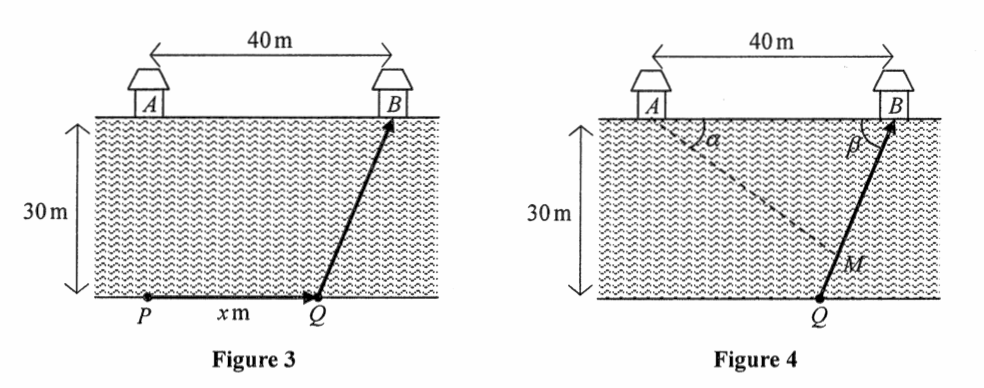
\includegraphics[width = \linewidth]{2013Figure3n4}
	\end{figure}
	\begin{enumerate}
		\item [(a)]Let $T$ seconds be the time that Mike travels from $P$ to $B$. 
		\begin{enumerate}
			\item [(i)]Express $T$ in terms of $x$. 
			\item [(ii)]When $T$ is minimum, show that $x$ satisfies the equation $2x^2 -160x+3125 = 0$. \\
			Hence show that $$QB = \displaystyle\frac{25\sqrt{6}}{2}\text{ m.}$$ (6 marks)
		\end{enumerate}
		\item [(b)]In Figure 4, Mike is swimming from $Q$ to $B$ with $QB$ equal to the value mentioned in (a)(ii).\\
		Let $\angle MAB = \alpha$ and $\angle ABM = \beta$, where $M$ is the position of Mike.
		\begin{enumerate}
			\item [(i)]By finding $\sin{\beta}$ and $\cos{\beta}$, show that $$MB = \displaystyle\frac{200\tan{\alpha}}{\tan{\alpha} + 2\sqrt{6}}.$$ 
			\item [(ii)]Find the rate of change of $\alpha$ when $\alpha = 0.2$ radian. Correct your answer to 4 decimal places.
		\end{enumerate}
		(7 marks)
	\end{enumerate}

	\item \textbf{HKDSE Math M2 2014 Q2}\\
	Consider the curve $C : y = x^3-3x$. 
	\begin{enumerate}
		\item [(a)]Find $\displaystyle\frac{dy}{dx}$ from  first principles. 
		\item [(b)]Find the range of $x$ where $C$ is decreasing.
	\end{enumerate}
	(5 marks)

	\item \textbf{HKDSE Math M2 2014 Q3}\\
	Find the equation of tangent to the curve $x\ln{y} + y = 2$ at the point where the curve cuts the $y$-axis.\\(5 marks)

	\item \textbf{HKDSE Math M2 2014 Q4}\\
	Let $x = 2y + \sin{y}$. Find $\displaystyle\frac{d^2y}{dx^2}$ in terms of $y$.\\(3 marks)

	\newpage

	\item \textbf{HKDSE Math M2 2014 Q10}\\
	Thomas has a bookcase of dimensions 100 cm $\times$ 24 cm $\times$ 192 cm at the corner in his room. He wants to hang a decoration on the wall above the bookcase. Therefore, he finds a ladder to climb up. Initially, the ladder touches the wall, the edge of the top of the bookcase and the floor at the same time. Let rectangle $ABCD$ be the side-view of the bookcase and $HK$ be the side-view of the ladder, so that $AB = 24$ cm and $BC = 192$ cm (see Figure 2). Let $\angle HKD = \theta$. 
	\begin{figure}[H]
		\centering
		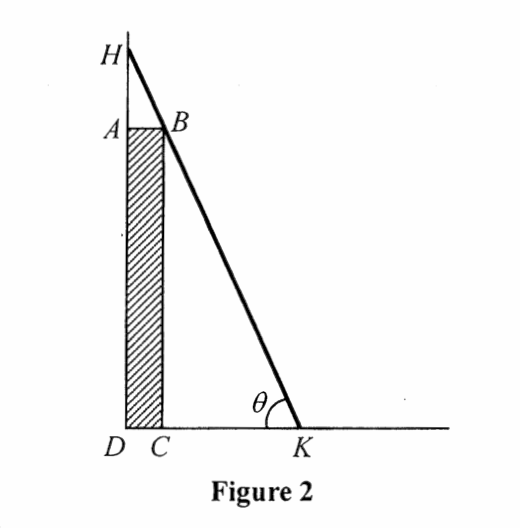
\includegraphics[width = .4\linewidth]{2014Figure2}
	\end{figure}
	\begin{enumerate}
		\item [(a)]Find the length of $HK$ in terms of $\theta$. \\(1 marks)
		\item [(b)]Prove that the shortest length of the ladder is $120\sqrt{5}$ cm. \\(5 marks)
		\item [(c)]
		Suppose the length of the ladder is 270 cm. Suddenly, the ladder slides down so that the end of the ladder, $K$, moves towards $E$ (see Figure 3). The ladder touches the edge of the top of the bookcase and the floor at the same time. Let $x$ cm and $y$ cm be the horizontal distances from $H$ and $K$ respectively to the wall.
		\begin{figure}[H]
			\centering
			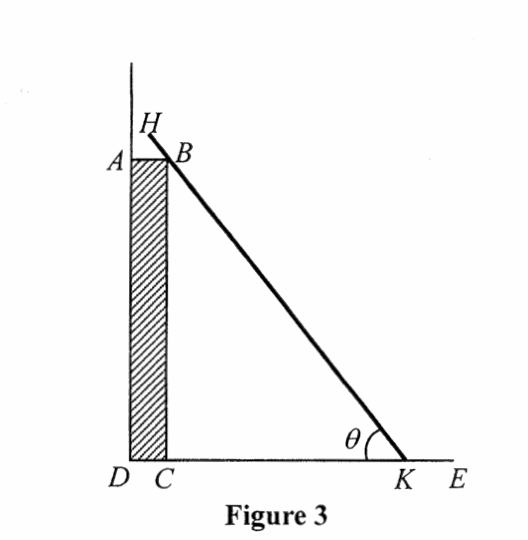
\includegraphics[width = .4\linewidth]{2014Figure3}
		\end{figure}
		\begin{enumerate}
			\item [(i)]When $CK = 160$ cm, the rate of change of $\theta$ is $-0.1$ rad s$^{-1}$. Find the rate of change of $x$ at this moment, \\correct to 4 significant figures. 
			\item [(ii)]Thomas claims that $K$ is moving towards $E$ at a speed faster than the horizontal speed $H$ is leaving the wall. Do you agree? Explain your answer.
		\end{enumerate}
		(6 marks)
	\end{enumerate}

	\newpage

	\item \textbf{HKDSE Math M2 2015 Q2}\\
	Let $y=x\sin{x} + \cos{x}$.  
	\begin{enumerate}
		\item [(a)]Find $\displaystyle\frac{dy}{dx}$ and $\displaystyle\frac{d^2y}{dx^2}$.
		\item [(b)]Let $k$ be a constant such that $x\displaystyle\frac{d^2y}{dx^2} + k\displaystyle\frac{dy}{dx} + xy = 0$ for all real values of $x$. Find the value of $k$.
	\end{enumerate}
	(5 marks)

	\item \textbf{HKDSE Math M2 2015 Q9}\\
	Define $f(x) = \displaystyle\frac{x^2+12}{x - 2}$ for all $x \neq 2$.  
	\begin{enumerate}
		\item [(a)]Find $f'(x)$. \\(2 marks)
		\item [(b)]Prove that the maximum value and the minimum value of $f(x)$ are $-4$ and $12$ respectively. \\(4 marks)
		\item [(c)]Find the asymptote(s) of the graph of $y = f(x)$. \\(3 marks) 
		\item [(d)]Find the area of the region bounded by the graph of $y = f(x)$ and the horizontal line $y = 14$.  \\(4 marks)
	\end{enumerate}

	\item \textbf{HKDSE Math M2 2016 Q3}\\
	Consider the curve $C : y = 2e^x$, where $x>0$. It is given that $P$ is a point lying on $C$. The horizontal line which passes through $P$ cuts the $y$-axis at the point $Q$. Let $O$ be the origin. Denote the $x$-coordinate of $P$ by $u$. 
	\begin{enumerate}
		\item [(a)]Express the area of $\triangle OPQ$ in terms of $u$.
		\item [(b)]If $P$ moves along $C$ such that $OQ$ increases at a constant rate of $6$ units per second, find the rate of change of the area of $\triangle OPQ$ when $u=4$.
	\end{enumerate}
	(5 marks)

	\item \textbf{HKDSE Math M2 2016 Q4}\\
	Define $f(x) = \displaystyle\frac{2x^2 + x + 1}{x - 1}$ for all $x \neq 1$. Denote the graph of $y = f(x)$ by $G$. Find 
	\begin{enumerate}
		\item [(a)]the asymptote(s) of $G$,
		\item [(b)]The slope of the normal to $G$ at the point $(2,11)$.
	\end{enumerate}
	(7 marks)

	\item \textbf{HKDSE Math M2 2016 Q9}\\
	Let $a$ and $b$ be constants. Define $f(x) = x^3 + ax^2 + bx + 5$ for all real numbers $x$. Denote the curve $y = f(x)$ by $C$. It is given that $P(-1,10)$ is a turning point of $C$.
	\begin{enumerate}
		\item [(a)]Find $a$ and $b$.\\(3 marks)
		\item [(b)]Is $P$ a maximum point of $C$? Explain your answer. \\(2 marks)
		\item [(c)]Find the minimum value(s) of $f(x)$. \\(2 marks)
		\item [(d)]Find the point(s) of inflexion of $C$. \\(2 marks)
		\item [(e)]Let $L$ be the tangent to $C$ at $P$. Find the area of the region bounded by $C$ and $L$. \\(4 marks)
	\end{enumerate}

	\newpage

	\item \textbf{HKDSE Math M2 2017 Q6}\\
	A container in the form of an inverted right circular cone is held vertically. The height and the base radius of the container are 20 cm and 15 cm respectively. Water is now poured into the container.
	\begin{enumerate}
		\item [(a)]Let $A$ cm$^2$ be the wet curve surface area of the container and $h$ cm be the depth of water in the container. Prove that $\displaystyle A = \frac{15}{16}\pi h^2$. 
		\item [(b)]The depth of water in the container increases at a constant rate of $\displaystyle\frac{3}{\pi}$ cm/s. Find the rate of change of the wet curved surface area of the container when the volume of water in the container is $96 \pi$ cm$^3$.
	\end{enumerate}
	(7 marks)

	\item \textbf{HKDSE Math M2 2017 Q8}\\
	Let $f(x) $ be a continuous function defined on  $\mathbb{R} ^+$, where $\mathbb{R} ^+$ is the set of positive real numbers. Denote the curve $y = f(x)$ by  $\Gamma$. It is given that $\Gamma$ passes through the point $P(e^3 , 7)$ and $f'(x) = \displaystyle\frac{1}{x} \ln{x^2}$ for all $x>0$. Find 
	\begin{enumerate}
		\item [(a)] the equation of the tangent to $\Gamma$ at $P$,
		\item [(b)] the equation of $\Gamma$,
		\item [(c)] the point(s) of inflexion of $\Gamma$.
	\end{enumerate}
	(8 marks)

	\item \textbf{HKDSE Math M2 2017 Q9}\\
	Define $f(x) = \displaystyle\frac{x^2 - 5x}{x + 4}$ for all $x \neq -4$. Denote the graph of $y = f(x)$ by $G$. 
	\begin{enumerate}
		\item [(a)]Find the asymptote(s) of $G$.  \\(3 marks)
		\item [(b)]Find $f'(x)$. \\(2 marks) 
		\item [(c)]Find the maximum point(s) and the minimum point(s) of $G$. \\(4 marks) 
		\item [(d)]Let $R$ be the region bounded by $G$ and the $x$-axis. Find the volume of the solid of revolution generated by revolving $R$ about the $x$-axis. \\(4 marks)
	\end{enumerate}

	\item \textbf{HKDSE Math M2 2018 Q8}\\
	Define $f(x) = \displaystyle \frac{A}{x^2-4x+7}$ for all real numbers $x$, where $A$ is a constant. \\
	It is given that the extreme value of $f(x)$ is 4. 
	\begin{enumerate}
		\item [(a)] Find $f'(x)$. 
		\item [(b)] Someone claims that there are at least two asymptotes of the graph of $ y =  f(x)$. Do you agree? \\
		Explain your answer. 
		\item [(c)] Find the point(s) of inflexion of the graph of $y =f(x)$.
	\end{enumerate}
	(8 marks)

	\item \textbf{HKDSE Math M2 2018 Q9}\\
	Consider the curve $C : y = \displaystyle\ln \sqrt{x}$, where $x > 1$. Let $P$ be a moving point lying on $C$. The normal to $C$ at $P$ cuts the $x$-axis at the point $Q$ while the vertical line passing through $P$ cuts the $x$-axis at the point $R$.  
	\begin{enumerate}
		\item [(a)]Denote the $x$-coordinate of $P$ by $r$. Prove that the $x$-coordinate of $Q$ is $\displaystyle\frac{4r^2+\ln r}{4r}$.  \\(3 marks)
		\item [(b)]Find the greatest area of $\triangle PQR$. \\(5 marks) 
		\item [(c)]Let $O$ be the origin. It is given that $OP$ increases at a rate not exceeding $32e^2$ units per minute. Someone claims that the area of $\triangle PQR$ increases at a rate lower than $2$ square units per minute when the $x$-coordinate of $P$ is $e$. Is the claim correct? Explain your answer. \\(4 marks) 
	\end{enumerate}

	\newpage

	\item \textbf{HKDSE Math M2 2019 Q3}\\
	A researcher performs an experiment to study the rate of change of the volume of liquid $X$ in a vessel. The experiment lasts for $24$ hours. At the start  of the experiment, the vessel contains $580 $cm$^3$ of liquid $X$. The researcher finds that during the experiment, $\displaystyle\frac{dV}{dt} = -2t$, where $V $cm$^3$ is the volume of liquid $X$ in the vessel and $t$ is the number of hours elapsed since the start of the experiment.
	\begin{enumerate}
		\item [(a)] The researcher claims that the vessel contains some liquid $X$ at the end of the experiment. \\
		Is the claim correct? Explain your answer.
		\item [(b)] It is given that $V = h^2+24h$, where $h $ cm is the depth of liquid $X$ in the vessel. \\
		Find the value of $\displaystyle\frac{dh}{dt}$ when $t = 18$.
	\end{enumerate}
	(6 marks)

	\item \textbf{HKDSE Math M2 2019 Q4}\\
	Define $\displaystyle g(x) = \frac{\ln{x}}{\sqrt{x}}$ for all $x \in (0,99)$. Denote the graph of $y = g(x) $ by $G$. 
	\begin{enumerate}
		\item [(a)]Prove that $G$ has only one maximum point. 
		\item [(b)]Let $R$ be the region bounded by $G$, the $x$-axis and the vertical line passing through the maximum point of $G$. Find the volume of the solid of revolution generated by revolving $R$ about the $x$-axis.
	\end{enumerate}
	(6 marks)

	\item \textbf{HKDSE Math M2 2019 Q8}\\
	Let $h(x)$ be a continuous function defined on $\mathbb{R}^+$, where $\mathbb{R}^+$ is the set of positive real numbers. It is given that $\displaystyle h'(x) = \frac{2x^2 -7x+8}{x}$ for all $x > 0$. 
	\begin{enumerate}
		\item [(a)] Is $h(x)$ an increasing function? Explain your answer. 
		\item [(b)] Denote the curve $y = h(x)$ by $H$. It is given that $H$ passes through the point $(1,3)$. Find  
		\begin{enumerate}
			\item [(i)]the equation of $H$,
			\item [(ii)]the point(s) of inflexion of $H$.
		\end{enumerate} 
	\end{enumerate}
	(8 marks)

	\item \textbf{HKDSE Math M2 2019 Q9}\\
	Consider the curve $\Gamma : y = \displaystyle\frac{1}{3}\sqrt{12-x^2}$, where $0<x<2\sqrt{3}$. Denote the tangent of $\Gamma$ at $x = 3$ by $L$.  
	\begin{enumerate}
		\item [(a)]Find the equation of $L$. \\(3 marks)
		\item [(b)]Let $C$ be the curve $y = \sqrt{4-x^2}$, where $0<x<2$. It is given that $L$ is a tangent to $C$. Find 
		\begin{enumerate}
			\item [(i)]the point(s) of contact of $L$ and $C$;  
			\item [(ii)]the point(s) of intersection of $C$ and $\Gamma$;  
			\item [(iii)]the area of region bounded by $L$, $C$ and $\Gamma$.
		\end{enumerate}
		(9 marks)
	\end{enumerate}

	\item \textbf{HKDSE Math M2 2020 Q6}\\
	Consider the curve $C_1 : y = 2^{x-1}$, where $x>0$. Denote the region by $O$. Let $P(u,v)$ be a moving point on $C_1$ such that the area of the circle with $OP$ as a diameter increases at a constant rate of $5\pi$ square units per second.
	\begin{enumerate}
		\item[(a)]
		Define $S = u^2 + v^2$. Does $S$ increase at a constant rate? Explain your answer. 
		\item[(b)]
		Let $C_2$ be the curve $y = 2^x$, where $x>0$. The vertical line passing through $P$ cuts $C_2$ at the point $Q$. Find the rate of change of the area of $\triangle OPQ$ when $u=2$.
	\end{enumerate}
	(7 marks)

	\newpage

	\item \textbf{HKDSE Math M2 2020 Q9}\\
	Let $\displaystyle f(x) = \frac{(x+4)^3}{(x-4)^2}$ for all real numbers $x \neq 4$. Denote the graph of $y = f(x)$ by $H$.
	\begin{enumerate}
		\item [(a)] Find the asymptote(s) of $H$. \\(3 marks)
		\item [(b)] Find $f''(x)$. \\(2 marks)
		\item [(c)] Someone claims that there are two turning points of $H$. Do you agree? Explain your answer. \\(2 marks)
		\item [(d)] Find the point(s) of inflexion of $H$. \\(2 marks)
		\item [(e)] Find the area of the region bounded by $H$, the $x$-axis and the $y$-axis. \\(3 marks)
	\end{enumerate}

	\item \textbf{HKDSE Math M2 2021 Q5}\\
	Define $\displaystyle r(x) = \frac{x^3 - x^2 -2x + 3}{(x-1)^2}$ for all real numbers $x \neq 1$.
	\begin{enumerate}
		\item [(a)] Find the asymptote(s) of the graph of $y = r(x)$.
		\item [(b)] Find $\displaystyle\frac{d}{dx}r(x)$.
		\item [(c)] Someone claims that there is only one point of inflexion of the graph of $y = r(x)$. Do you agree? \\
		Explain your answer.
	\end{enumerate}
	(7 marks)

	\item \textbf{HKDSE Math M2 2021 Q6}\\
	Consider the curve $\Gamma : y = e^{2x-6}$. Denote the normal to $\Gamma$ at the point $(3,1)$ by $L$. \\
	Let $c$ be the $x$-intercept of $L$. Find
	\begin{enumerate}
		\item [(a)]$c$;
		\item [(b)]the area of the region bounded by $L$, $\Gamma$ and the straight line $x=c$.
	\end{enumerate}
	(7 marks)

	\item \textbf{HKDSE Math M2 2021 Q10}\\
	Denote the graph of $y = \sqrt{x^2+36} $ and the graph of $y = - \sqrt{(20-x)^2+16}$ by $F$ and $G$ respectively, where $0 < x<20$. Let $P$ be a moving point on $F$. The vertical line passing through $P$ cuts $G$ at the point $Q$. Denote the $x$-coordinate of $P$ by $u$. It is given that the length of $PQ$ attains its minimum value when $u=a$.
	\begin{enumerate}
		\item [(a)] Find $a$.\\(4 marks)
		\item [(b)] The horizontal line passing through $P$ cuts the $y$-axis at the point $R$ while the horizontal line passing through $Q$ cuts the $y$-axis at the point $S$.
		\begin{enumerate}
			\item [(i)] Someone claims that the area of the rectangle $PQSR$ attains its minimum value when $u = a$. Do you agree? Explain your answer. 
			\item [(ii)] The length of $OP$ increases at a constant rate of 28 units per minute. Find the rate of change of the perimeter of the rectangle $PQSR$ when $u = a$.
		\end{enumerate}
		(9 marks)
	\end{enumerate}

	\newpage

	\item \textbf{HKDSE Math M2 2022 Q4}\\
	Let $y = (7x - 2x^2)e^{-x}$.
	\begin{enumerate}
		\item[(a)]
		Find $\displaystyle \frac{dy}{dx}$ and $\displaystyle \frac{d^2y}{dx^2}$. 
		\item[(b)]
		Someone claims that there are two points of inflexion of the graph of $y = (7x - 2x^2)e^{-x}$. \\
		Do you agree? Explain your answer. 
	\end{enumerate}
	(6 marks)

	\item \textbf{HKDSE Math M2 2022 Q7}\\
	Consider the curve $\Gamma : y = \ln{(x+2)}$, where $x > 0$. Let $P$ be a moving point on $\Gamma$ with $h$ as its $x$-coordinate. Denote the tangent to $\Gamma$ at $P$ by $L$ and the area of the region bounded by $\Gamma$, $L$ and the $y$-axis by $A$ square units.
	\begin{enumerate}
		\item [(a)]Prove that $\displaystyle A = \frac{h^2+4h}{2h+4} - 2\ln{(h+2)} + 2\ln{2}$.
		\item [(b)]If $h = 3^{-t}$, where $t$ is the time measured in seconds, find the rate of change of $A$ when $t = 1$.
	\end{enumerate}
	(8 marks)

	\item \textbf{HKDSE Math M2 2022 Q9}\\
	Let $\displaystyle f(x) = \frac{x^2 +3x}{x-1}$, where $x \neq 1$. Denote the graph of $y = f(x)$ by $H$.
	\begin{enumerate}
		\item [(a)] Find the asymptote(s) of $H$. \\(3 marks)
		\item [(b)] Find the maximum point(s) and minimum point(s) of $H$. \\(4 marks)
		\item [(c)] Sketch $H$. \\(3 marks)
		\item [(d)] Let $R$ be the region bounded by $H$ and the straight line $y = 10$. Find the volume of the solid of revolution generated by revolving $R$ about the straight line $y = 10$. \\(3 marks)
	\end{enumerate}

	\item \textbf{HKDSE Math M2 2023 Q6}
	\begin{enumerate}
		\item [(a)]Let $r$ be a positive constant. Figure 1 shows the shaded region which is inside the circle $x^2 + (y-r)^2 = r^2$ and below the horizontal line $y = h$, where $0 \leq h \leq 2r$. Prove that the volume of the solid of revolution generated by revolving the shaded region about the $y$-axis is $\dfrac{\pi}{3}h^2(3r-h)$.
		\begin{figure}[H]
			\centering
			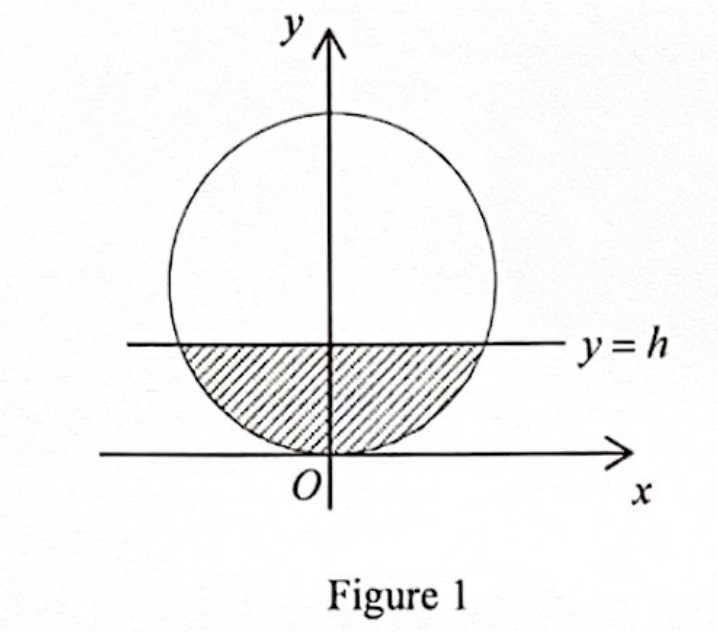
\includegraphics[width = .5\linewidth]{2023Figure1}
		\end{figure}
		\item [(b)]A solid metal sphere of radius 10 cm is put into an empty right cylindrical container of radius 11 cm and height 20 cm, with longitudinal section as shown in Figure 2. Starting from time $t=0$, water is added to the container at a constant rate of 1 cm$^3$ per second. Let $h$ cm be the depth of water after $t$ seconds. By expressing $\dfrac{\text{d}h}{\text{d}t}$ in terms of $h$, find the greatest value of $\dfrac{\text{d}h}{\text{d}t}$.
		\begin{figure}[H]
			\centering
			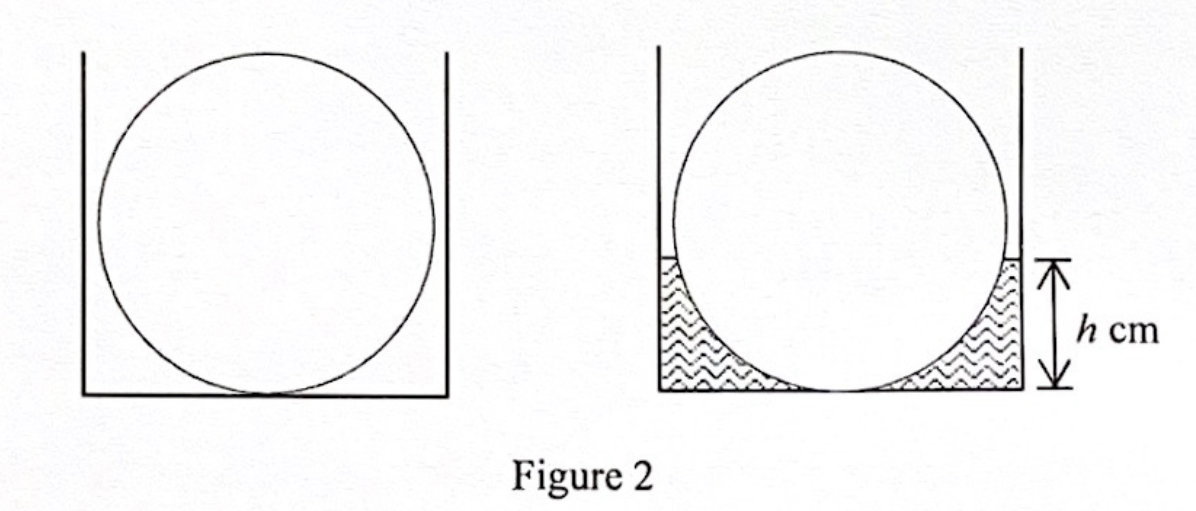
\includegraphics[width = .5\linewidth]{2023Figure2}
		\end{figure}
	\end{enumerate}
	(7 marks)

	\item \textbf{HKDSE Math M2 2023 Q7}\\
	Let $f(x)$ be a function defined on the interval $(-2,2)$. Denote the curve $y = f(x)$ by $\Gamma$. At any point $(x,y)$ on $\Gamma$, the slope of the tangent to $\Gamma$ is $\dfrac{k - 3x}{\sqrt{4-x^2}}$, where $k$ is a constant. It is given that $\Gamma$ passes through the origin.
	\begin{enumerate}
		\item [(a)]Find the equation of $\Gamma$ in terms of $k$.
		\item [(b)]Suppose that $\Gamma$ has a turning point.
		\begin{enumerate}
			\item [(i)]Find the range of values of $k$.
			\item [(ii)]Does $\Gamma$ have a point of inflexion? Explain your answer.
		\end{enumerate}
	\end{enumerate}
	(7 marks)

	\item \textbf{HKDSE Math M2 2023 Q9}\\
	Define $ f(x) = xe^{-x^2}$ for all $x\in \mathbb{R}$. Denote the graph of $y = f(x)$ by $G$.
	\begin{enumerate}
		\item [(a)]Find $f'(x)$ and $f''(x)$. \\(3 marks)
		\item [(b)]Find the maximum point(s) and minimum point(s) of $G$. \\(3 marks)
		\item [(c)]Let $L$ be the tangent to $G$ at the point $\left(1,\dfrac{1}{e}\right)$.
		\begin{enumerate}
			\item [(i)]Find the equation of $L$.
			\item [(ii)]By considering $f''(x)$, explain why $G$ lies below $L$ in the interval $(0,1)$.
			\item [(iii)]Find the area of the region bounded by $G$, $L$ and the $y$-axis.
		\end{enumerate}
		(6 marks)
	\end{enumerate}
\end{enumerate}

\chapter{Technique of Integration}
\begin{enumerate}
	\item \textbf{HKDSE Math M2 Sample Paper Q4}\\
	Find $\displaystyle\int\left(x^2-\frac{1}{x}\right)^4 \,dx$. \\(4 marks)

	\item \textbf{HKDSE Math M2 Sample Paper Q8}
	\begin{enumerate}
		\item [(a)]Using integration by parts, find $\displaystyle\int x\cos{x}\,dx$. 
		\item [(b)]The \textbf{inner surface} of a container is formed by revolving the curve $y = -\cos{x}$ (for $0 \leq x \leq \pi$) about the $y$-axis (see Figure 1). Find the capacity of the container. \\(6 marks)
		\begin{figure}[H]
			\centering
			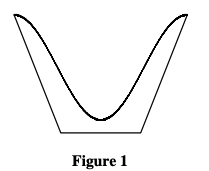
\includegraphics[width = .3\linewidth]{SPFigure1}
		\end{figure}
	\end{enumerate}

	\item \textbf{HKDSE Math M2 Sample Paper Q13}
	\begin{enumerate}
		\item[(a)]Let $a > 0$ and $f(x)$ be a continuous function. Prove that $$\displaystyle\int_{0}^a f(x) \,dx = \int_{0}^a f(a-x) \,dx.$$
		Hence, prove that $$\displaystyle\int_{0}^a f(x) \,dx = \frac{1}{2}\int_{0}^a [f(x) + f(a-x)] \,dx.$$ \\(3 marks)
		\item[(b)]Show that $$\displaystyle\int_0^1 \frac{dx}{x^2-x+1} = \frac{2\sqrt{3}\pi}{9}.$$ \\(5 marks)
		\item[(c)]Using (a) and (b), or otherwise, evaluate $\displaystyle\int_0^1 \frac{dx}{(x^2-x+1)(e^{2x-1}+1)}$. \\(6 marks)
	\end{enumerate}

	\newpage

	\item \textbf{HKDSE Math M2 Practice Paper Q8}
	\begin{enumerate}
		\item [(a)]Using integration by substitution, find $\displaystyle\int\frac{dx}{\sqrt{4-x^2}}$. 
		\item [(b)]Using integration by parts, find $\displaystyle\int\ln{x}\,dx$.
	\end{enumerate}
	(5 marks)

	\item \textbf{HKDSE Math M2 Practice Paper Q10}
	\begin{enumerate}
		\item [(a)]Find $\displaystyle\int xe^{-x^2} \,dx$. 
		\item [(b)]In Figure 1, the shaded region is bounded by the curves $y = \displaystyle\frac{x^2}{2}$ and $y = e^{-x^2}$, where $1 \leq x \leq 2$. Find the volume of the solid generated by revolving the shaded region about the $y$-axis.\\
	(6 marks)
		\begin{figure}[H]
			\centering
			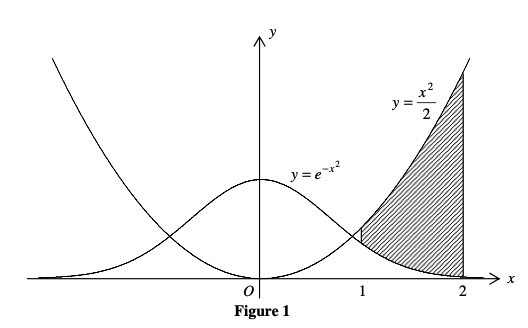
\includegraphics[width = .5\linewidth]{PPFigure1}
		\end{figure}
	\end{enumerate}

	\item \textbf{HKDSE Math M2 Practice Paper Q13}
	\begin{enumerate}
		\item[(a)]Let $f(x)$ be an odd function for $-p \leq x \leq p$, where $p$ is a positive constant.
		Prove that $$\displaystyle\int_0^{2p} f(x-p)\,dx = 0.$$
		Hence evaluate $\displaystyle\int_0^{2p} [f(x-p)+q]\,dx $, where $q$ is a constant. \\(4 marks)
		\item[(b)]Prove that $$\displaystyle\frac{\sqrt{3} + \tan{\left(x - \displaystyle\frac{\pi}{6}\right)}}{\sqrt{3} - \tan{\left(x - \displaystyle\frac{\pi}{6}\right)}} = \frac{1+\sqrt{3}\tan{x}}{2}.$$ \\(2 marks)
		\item[(c)]Using (a) and (b), or otherwise, evaluate $\displaystyle\int_0^{\tfrac{\pi}{3}} \ln{(1 + \sqrt{3}\tan{x})} \,dx$. \\(4 marks)
	\end{enumerate}

	\item \textbf{HKDSE Math M2 2012 Q4}
	\begin{enumerate}
		\item [(a)]Find $\displaystyle\int \frac{x+1}{x}\,dx$
		\item [(b)]Using the substitution $u = x^2-1$, find $\displaystyle\int\frac{x^3}{x^2 - 1}\,dx$.
	\end{enumerate}
	(5 marks)

	\newpage

	\item \textbf{HKDSE Math M2 2012 Q9}
	\begin{enumerate}
		\item [(a)]Using integration by parts, find $\int x\sin{x}\,dx$. 
		\item [(b)]Figure 4 shows the shaded region bounded by the curve $y = \sqrt{x\sin{x}}$ for $0 \leq x \leq \pi$ and the $x$-axis. Find the volume of the solid generated by revolving the region about the $x$-axis.
	\begin{figure}[H]
		\centering
		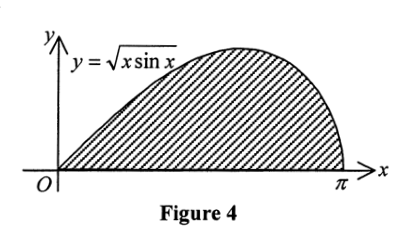
\includegraphics[width = .5\linewidth]{2012Figure4}
	\end{figure}
	\end{enumerate}
	(4 marks)

	\item \textbf{HKDSE Math M2 2012 Q13}
	\begin{enumerate}
		\item [(a)]
		\begin{enumerate}
			\item [(i)]Suppose $\tan{u} = \displaystyle\frac{-1 + \cos{\displaystyle\frac{2\pi}{5}}}{\sin{\displaystyle\frac{2\pi}{5}}}$, where $\displaystyle\frac{-\pi}{2} < u < \frac{\pi}{2}$. \\
			Show that $u = \displaystyle\frac{-\pi}{5}$. 
			\item [(ii)]Suppose $\tan{v} = \displaystyle\frac{1+\cos{\displaystyle\frac{2\pi}{5}}}{\sin{\displaystyle\frac{2\pi}{5}}}$. \\
			Find $v$, where $\displaystyle\frac{-\pi}{2} < v < \frac{\pi}{2}$.
		\end{enumerate}
		(4 marks)
		\item[(b)]
		\begin{enumerate}
			\item[(i)]Express $x^2 + 2x\cos{\displaystyle\frac{2\pi}{5}} + 1$ in the form $(x+a)^2 + b^2$, where $a$ and $b$ are constants. 
			\item[(ii)]Evaluate $\displaystyle\int_{-1}^{1}\frac{\sin{\displaystyle\frac{2\pi}{5}}}{x^2 + 2x\cos{\displaystyle\frac{2\pi}{5}}+1}\, dx$.
		\end{enumerate}
		(6 marks)
		\item[(c)]Evaluate $\displaystyle\int_{-1}^{1}\frac{\sin{\displaystyle\frac{7\pi}{5}}}{x^2 + 2x\cos{\displaystyle\frac{7\pi}{5}}+1} \,dx$. \\(3marks)
	\end{enumerate}

	\newpage

	\item \textbf{HKDSE Math M2 2013 Q11}
	\begin{enumerate}
		\item [(a)]Let $0 < \theta < \displaystyle\frac{\pi}{2}$. By finding $\displaystyle\frac{d}{d\theta} \ln{(\sec{\theta} + \tan{\theta})}$, or otherwise, show that $$\displaystyle\int\sec{\theta}\,d\theta =\ln{(\sec{\theta} + \tan{\theta})} + C,$$where $C$ is any constant. \\(2 marks)
		\item [(b)]
		\begin{enumerate}
			\item [(i)]Using (a) and a suitable substitution, show that $$\displaystyle\int\frac{du}{\sqrt{u^2-1}} = \ln{(u + \sqrt{u^2-1})} + C$$ for $u > 1$.
			\item [(ii)]Using (b)(i), show that $$\displaystyle\int_{0}^{1}\frac{2x}{\sqrt{x^4+4x^2+3}}\,dx = \ln{(6 + 4\sqrt{2} - 3\sqrt{3} - 2\sqrt{6})}.$$
		\end{enumerate}
		(5 marks)
		\item [(c)]Let $t = \tan{\phi}$. Show that $$\displaystyle\frac{d\phi}{dt} = \frac{1}{1+t^2}.$$ \\
		Hence evaluate $\displaystyle\int_0^{\tfrac{\pi}{4}}\frac{\tan{\phi}}{\sqrt{1+2\cos^2{\phi}}}\,d\phi$. \\(5 marks)
	\end{enumerate}

	\item \textbf{HKDSE Math M2 2014 Q5}
	\begin{enumerate}
		\item [(a)]Find $\displaystyle\int \frac{dx}{\sqrt{9-x}}$, where $x < 9$. 
		\item [(b)]Using integration by substitution, find $\displaystyle\int \frac{dx}{\sqrt{9-x^2}}$, where $-3 < x < 3$.
	\end{enumerate}
	(6 marks)

	\item \textbf{HKDSE Math M2 2014 Q6}
	\begin{enumerate}
		\item [(a)]Find $\displaystyle\int xe^{-x}\,dx$. 
		\item [(b)]Figure 1 shows the shaded region bounded by the curve $y = xe^{-x}$ and the straight line $y = \displaystyle\frac{x}{e}$. \\
		Find the area of the shaded region.
		\begin{figure}[H]
			\centering
			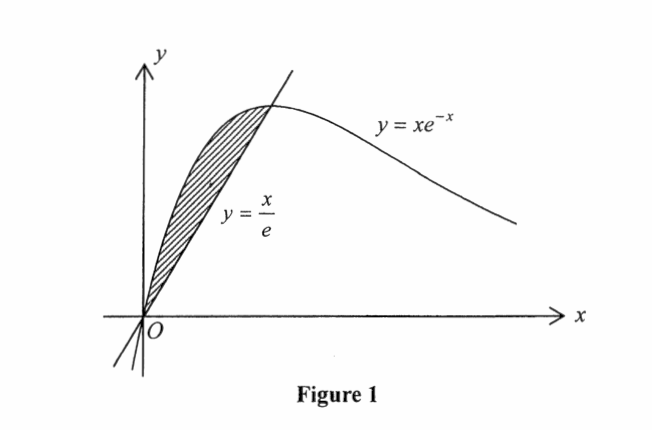
\includegraphics[width = .5\linewidth]{2014Figure1}
		\end{figure}
	\end{enumerate}
	(6 marks)

	\newpage

	\item \textbf{HKDSE Math M2 2015 Q3}
	\begin{enumerate}
		\item [(a)]Find $\displaystyle\int \frac{1}{e^{2u}} \,du$. 
		\item [(b)]Using integration by substitution, evaluate $\displaystyle\int_1^9 \frac{1}{\sqrt{x}e^{2\sqrt{x}}}\,dx$. 
	\end{enumerate}
	(7 marks)

	\item \textbf{HKDSE Math M2 2015 Q4}
	\begin{enumerate}
		\item [(a)]Using integration by parts, find $\displaystyle\int x^2 \ln{x} \,dx $. 
		\item [(b)]At any point $(x,y)$ on the curve $\Gamma $, the slope of the tangent to $\Gamma$ is $9x^2 \ln{x}$. It is given that $\Gamma$ passes through the point $(1,4)$. Find the equation of $\Gamma$.  
	\end{enumerate}
	(7 marks)	

	\item \textbf{HKDSE Math M2 2016 Q7}
	\begin{enumerate}
		\item [(a)]Using integration by substitution, find $\displaystyle\int (1+\sqrt{t+1})^2 \,dt$. 
		\item [(b)]Consider the curve $\Gamma : y = 4x^2 - 4x$, where $1 \leq x \leq 4$. Let $R$ be the region bounded by $\Gamma$, the straight line $y=48$ and the two axes. Find the volume of the solid of revolution generated by revolving $R$ about the $y$-axis.
	\end{enumerate}
	(8 marks)

	\item \textbf{HKDSE Math M2 2016 Q10}
	\begin{enumerate}
		\item [(a)]Let $f(x)$ be a continuous function defined on the interval $[0,a]$, where $a$ is a positive constant. \\Prove that $\displaystyle\int_0^a f(x)\,dx = \int_0^a f(a-x)\,dx$. \\(3 marks)
		\item [(b)]Prove that $$\displaystyle\int_{0}^{\tfrac{\pi}{4}} \ln{(1+\tan{x})}\,dx = \int_{0}^{\tfrac{\pi}{4}} \ln{\left(\frac{2}{1+\tan{x}}\right)}\,dx.$$ \\(3 marks)
		\item [(c)]Using (b), prove that $$\displaystyle\int_{0}^{\tfrac{\pi}{4}} \ln {(1+\tan{x})}\,dx = \frac{\pi \ln 2}{8}.$$ \\(3 marks)
		\item [(d)]Using integration by parts, evaluate $\displaystyle\int_{ 0}^{\tfrac{\pi}{4}} \frac{x\sec^2{x}}{1+\tan{x}}\,dx$. \\(3 marks)
	\end{enumerate}

	\item \textbf{HKDSE Math M2 2017 Q4}	
	\begin{enumerate}
		\item [(a)]Using integration by parts, find $\displaystyle\int x^2 e^{-x} \,dx$. 
		\item [(b)]Find the area of the region bounded by the graph of $y = x^2 e^{-x}$, the $x$-axis and the straight line $x = 6$.
	\end{enumerate}
	(6 marks)
	
	\newpage

	\item \textbf{HKDSE Math M2 2017 Q11}
	\begin{enumerate}
		\item [(a)]Using $\displaystyle\tan^{-1}{\sqrt{2}} - \tan^{-1}{\left(\frac{\sqrt{2}}{2}\right)} = \tan^{-1}{\left(\frac{\sqrt{2}}{4}\right)}$, evaluate $\displaystyle\int_{0}^{1} \frac{1}{x^2+2x+3}\,dx $. \\(3 marks)
		\item [(b)]
		\begin{enumerate}
			\item [(i)]Let $0 \leq \theta \leq \displaystyle\frac{\pi}{4}$ . Prove that $\displaystyle\frac{2\tan{\theta}}{1 + \tan^2{\theta}} = \sin{2\theta}$ and $\displaystyle\frac{1-\tan^2{\theta}}{1 + \tan^2{\theta}} = \cos{2\theta}$.
			\item [(ii)]Using the substitution $t = \tan{\theta}$, evaluate $\displaystyle\int_{0}^{\tfrac{\pi}{4}} \frac{1}{\sin{2\theta} + \cos{2\theta} + 2} \,d\theta$.
		\end{enumerate}
		(5 marks)
		\item [(c)]Prove that $$\displaystyle\int_{0}^{\tfrac{\pi}{4}} \frac{\sin{2\theta}+1 }{\sin{2\theta} + \cos{2\theta} + 2} \,d\theta = \displaystyle\int_{0}^{\tfrac{\pi}{4}} \frac{\cos{2\theta}+1}{\sin{2\theta} + \cos{2\theta} + 2} \,d\theta.$$(2 marks)
		\item [(d)]Evaluate $\displaystyle\int_{0}^{\tfrac{\pi}{4}} \frac{8\sin{2\theta} + 9}{\sin{2\theta} + \cos{2\theta} + 2} \,d\theta$. \\(3 marks)
	\end{enumerate}

	\item \textbf{HKDSE Math M2 2018 Q4}
	\begin{enumerate}
		\item [(a)]Using integration by parts, find $\displaystyle\int u(5^u) \,du$. 
		\item [(b)]Define $f(x) = x(5^{2x})$ for all real numbers $x$. Find the area of the region bounded by the graph of $y = f(x)$, the straight line $x = 1$ and the $x$-axis.
	\end{enumerate}
	(6 marks)
	
	\item \textbf{HKDSE Math M2 2018 Q10}
	\begin{enumerate}
		\item [(a)] 
		\begin{enumerate}
			\item [(i)]Prove that $$\displaystyle \int \sin^4{x}\,dx = \frac{-\cos{x}\sin^3{x}}{4} + \frac{3}{4} \int \sin^2{x} \,dx.$$ 
			\item [(ii)] Evaluate $\displaystyle \int_{0}^{\pi} \sin^4{x}\,dx$.
		\end{enumerate}
		(5 marks)
		\item [(b)] 
		\begin{enumerate}
			\item [(i)]Let $f(x)$ be a continuous function such that $f(\beta - x)= f(x)$ for all real numbers $x$, where $\beta$ is a constant. Prove that $$\displaystyle\int_{0}^{\beta} x f(x) \,dx = \frac{\beta}{2} \int_{0}^{\beta } f(x) \,dx.$$
			\item [(ii)] Evaluate $\displaystyle \int_{0}^{\pi} x\sin^4{x}\,dx$.
		\end{enumerate}
		(5 marks)
	\item [(c)]Consider the curve $G : y = \displaystyle \sqrt{x}\sin^2{x}$, where $\pi \leq x \leq 2\pi $.
	Let $R$ be the region bounded by $G$ and the $x$-axis.
	Find the volume of the solid of revolution generated by revolving $R$ about the $x$-axis. \\(3 marks) 
	\end{enumerate}

	\item \textbf{HKDSE Math M2 2019 Q7}
	\begin{enumerate}
		\item [(a)]Using integration by parts, find $\displaystyle\int e^x\sin{\pi x}\, dx$. 
		\item [(b)]Using integration by substitution, evaluate $\displaystyle\int_{0}^{3} e^{3-x}\sin{\pi x} \,dx$.
	\end{enumerate}
	(7 marks)
	
	\newpage

	\item \textbf{HKDSE Math M2 2019 Q10}
	\begin{enumerate}
		\item [(a)] Let $0 \leq x \leq \displaystyle\frac{\pi}{4}$. Prove that $\displaystyle\frac{1}{2+\cos{2x}} = \frac{\sec^2{x}}{2+\sec^2{x}}$. \\(1 mark) 
		\item [(b)] Evaluate $\displaystyle \int_{0}^{ \tfrac{\pi}{4}} \frac{1}{2+\cos{2x}}\,dx$. \\(3 marks)
		\item [(c)] Let $f(x)$ be a continuous function defined on $\mathbb{R}$ such that $f(-x) = -f(x)$ for all $x \in \mathbb{R}$. Prove that $$\displaystyle\int_{-a}^{a} f(x)\ln{(1+e^x)}\,dx = \int_{0}^{a} xf(x)\,dx$$ for any $a \in \mathbb{R}  $. \\(4 marks)
		\item [(d)] Evaluate $\displaystyle \int_{\tfrac{-\pi}{4}}^{\tfrac{\pi}{4}}  \frac{\sin{2x}}{(2+\cos{2x})^2}\ln(1 + e^x)\,dx$. \\(5 marks)
	\end{enumerate}

	\item \textbf{HKDSE Math M2 2020 Q4}
	\begin{enumerate}
		\item [(a)]Find $\displaystyle \int \sin^2{\theta} \,d\theta$. 
		\item [(b)]Define $\displaystyle f(x) = 4x(1-x^2)^{\frac{1}{4}}$ for all $x \in [0,1]$. Denote the graph of $y = f(x) $ by $G$. \\
		Let $R$ be the region bounded by $G$ and the $x$-axis. \\
		Find the volume of the solid of revolution generated by revolving $R$ about the $x$-axis.
	\end{enumerate}
	(6 marks)

	\item \textbf{HKDSE Math M2 2020 Q10}
	\begin{enumerate}
		\item [(a)]Using integration by substitution, prove that $$\displaystyle \int_{\tfrac{\pi}{12}}^{\tfrac{\pi}{6}}  \ln{\left(\sin{\left(\frac{\pi}{4} - x\right)}\right)}\,dx = \int_{\tfrac{\pi}{12}}^{\tfrac{\pi}{6}}  \ln{(\sin{x})}\,dx.$$ \\(3 marks)
		\item [(b)] Using (a), evaluate $\displaystyle \int_{\tfrac{\pi}{12}}^{\tfrac{\pi}{6}}  \ln{(\cot{x} - 1)}\,dx$. \\(3 marks)
		\item [(c)] 
		\begin{enumerate}
			\item [(i)] Using $\cot{(A-B)} = \displaystyle \frac{\cot{A}\cot{B}+1}{\cot{B} - \cot{A}}$, or otherwise, prove that $\displaystyle \cot{\frac{\pi}{12}} = 2 + \sqrt{3}$. 
			\item [(ii)] Using integration by parts, prove that $$\displaystyle\int_{\tfrac{\pi}{12}}^{\tfrac{\pi}{6}}  \frac{x\csc^2{x}}{\cot{x} -1}\,dx = \frac{\pi}{8} \ln{(2 + \sqrt{3})}.$$
		\end{enumerate}
	    (7 marks)
	\end{enumerate}

	\item \textbf{HKDSE Math M2 2021 Q7}
	\begin{enumerate}
		\item [(a)]Using integration by parts, find $\displaystyle\int (\ln{x})^2 \,dx$.
		\item [(b)] Consider the curve $\displaystyle C : y = \sqrt{x}\ln{(x^2+1)}$, where $x\geq 0$. Let $R$ be the region bounded by $C$, the straight line $x=1 $ and the $x$-axis. Find the volume of the solid of revolution generated by revolving R about the $x$-axis.
	\end{enumerate}
	(7 marks)

	\newpage

	\item \textbf{HKDSE Math M2 2021 Q9}
	\begin{enumerate}
		\item [(a)] Let $\displaystyle \frac{-\pi}{2} < \theta < \frac{\pi}{2}$.
		\begin{enumerate}
			\item [(i)] Find $\displaystyle \frac{d}{d\theta} \ln{(\sec{\theta} + \tan{\theta})}$.
			\item [(ii)] Using the result of (a)(i), find $\displaystyle \int \sec{\theta} \,d\theta$. Hence, find $\displaystyle \int \sec^3{\theta}\,d\theta$. 
		\end{enumerate}
		(4 marks)
		\item [(b)] Let $g(x)$ and $h(x)$ be continuous functions defined on $\mathbb{R}$ such that $g(x)+g(-x) =1$ and $h(x)=h(-x) $ for all $x \in \mathbb{R}$. \\Using integration by substitution, prove that $\displaystyle\int_{-a}^{a}g(x)h(x)\,dx = \int_{0}^{a}h(x)\,dx$ for any $a \in \mathbb{R}$.\\(3 marks)
		\item Evaluate $\displaystyle \int_{-1}^{1} \frac{3^x x^2}{(3^x+3^{-x})\sqrt{x^2+1}}\,dx$.\\(5 marks)
	\end{enumerate}

	\item \textbf{HKDSE Math M2 2022 Q6}
	\begin{enumerate}
		\item [(a)]Using integration by substitution, prove that $$\displaystyle \int \frac{1}{x^2+2x+5}\,dx = \frac{1}{2} \tan^{-1} \left(\frac{x+1}{2}\right) +\text{ constant.}$$
		\item [(b)]At any point $(x,y)$ on the curve $G$, the slope of the tangent to $G$ is $\displaystyle \frac{2x+1}{x^2+2x+5}$.\\
		Given that $G$ passes through the point $(-3, \ln{2})$, does $G$ pass through the point $\displaystyle \left(-1, \frac{-\pi}{8}\right)$? \\
		Explain your answer.
	\end{enumerate}
	(7 marks)

	\item \textbf{HKDSE Math M2 2022 Q6}
	\begin{enumerate}
		\item [(a)]Using integration by substitution, prove that $$\displaystyle \int \frac{1}{x^2+2x+5}\,dx = \frac{1}{2} \tan^{-1} \left(\frac{x+1}{2}\right) +\text{ constant.}$$
		\item [(b)]At any point $(x,y)$ on the curve $G$, the slope of the tangent to $G$ is $\displaystyle \frac{2x+1}{x^2+2x+5}$.\\
		Given that $G$ passes through the point $(-3, \ln{2})$, does $G$ pass through the point $\displaystyle \left(-1, \frac{-\pi}{8}\right)$? \\
		Explain your answer.
	\end{enumerate}
	(7 marks)

	\item \textbf{HKDSE Math M2 2022 Q10}\\
	Let $g(x) = \cos^2{x}\cos{2x}$.
	\begin{enumerate}
		\item [(a)] Prove that $\displaystyle \int g(x) \,dx = \frac{\sin{2x}\cos^2{x}}{2} + \frac{1}{2} \int \sin^2{2x}\,dx$. \\(2 marks)
		\item [(b)] Evaluate $\displaystyle \int_{0}^{\pi} g(x) \,dx$. \\(2 marks)
		\item [(c)] Using integration by substitution, evaluate $\displaystyle \int_{0}^{\pi} xg(x) \,dx$. \\(4 marks)
		\item [(d)] Evaluate $\displaystyle \int_{-\pi}^{2\pi} xg(x) \,dx$. \\(4 marks)
	\end{enumerate}

	\item \textbf{HKDSE Math M2 2023 Q3}
	\begin{enumerate}
		\item [(a)]Find a pair of constants $p$ and $q$ such that $$11\sin{x} + 7\cos{x} \equiv p(3\sin{x} + \cos{x}) + q(3\cos{x} - \sin{x}).$$
		\item [(b)]Evaluate $\displaystyle \int^{\frac{\pi}{4}}_{0} \dfrac{11\sin{x} + 7\cos{x}}{3\sin{x} + \cos{x}} \,dx$.
	\end{enumerate}
	(6 marks)

	\item \textbf{HKDSE Math M2 2023 Q11}
	\begin{enumerate}
		\item [(a)] Consider the system of linear equations in real variables $x$, $y$, $z$
		$$(E) : \left\{\begin{matrix}
		x&	+&	ay&		+&	(a+1)z&		=&	2  \\
		x&	+&	(a+4)y&	+&	(2a+4)z&	=&	b+1 \\
		2x&	+&	3y&		+&	5z&			=&	b \\
		\end{matrix}\right. \text{,  where } a, b \in \mathbb{R} .$$
		\begin{enumerate}
			\item [(i)] Assume that $(E)$ has a unique solution. Find the range of values of $a$.
			\item [(ii)] Assume that $a = 1$. If $(E)$ is consistent, find $b$.
			\item [(iii)] Assume that $a \neq 1$ and $(E)$ is incnsistent. Find the range of values of $b$.
		\end{enumerate}
		(7 marks)
		\item [(b)] Consider the system of linear equations in real variables $x$, $y$, $z$
		$$(F) : \left\{\begin{matrix}
		x&	+&	2y&	+&	3z&	=&	2  \\
		x&	+&	6y&	+&	8z&	=&	s+1 \\
		2x&	+&	3y&	+&	5z&	=&	s \\
		\end{matrix}\right. \text{,  where } s \in \mathbb{R} .$$
		Does there exist a pair of real constants $m$ and $n$ (independent of $s$) such that for every $s\in\mathbb{R}$, $(F)$ has a real solution $(x,y,z)$ satisfying $mx + ny + z = -2$? Explain your answer. \\(6 marks) 
	\end{enumerate}

\end{enumerate}

\chapter{Applications of Integration}
\begin{enumerate}
	\item \textbf{HKDSE Math M2 Sample Paper Q3}\\
	The slope at any point $(x,y)$ of a curve is given by $\displaystyle\frac{dy}{dx} = 2x \ln{(x^2+1)}$. It is given that the curve passes through the point $(0,1)$.\\Find the equation of the curve. \\(4 marks)

	\item \textbf{HKDSE Math M2 Sample Paper Q8}
	\begin{enumerate}
		\item [(a)]Using integration by parts, find $\displaystyle\int x\cos{x}\,dx$. 
		\item [(b)]The \textbf{inner surface} of a container is formed by revolving the curve $y = -\cos{x}$ (for $0 \leq x \leq \pi$) about the $y$-axis (see Figure 1). Find the capacity of the container. \\(6 marks)
		\begin{figure}[H]
			\centering
			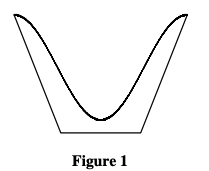
\includegraphics[width = .3\linewidth]{SPFigure1}
		\end{figure}
	\end{enumerate}
	
	\item \textbf{HKDSE Math M2 Sample Paper Q12}\\
	Let $\displaystyle f(x) = \frac{4}{x-1} - \frac{4}{x+1} -1$, where $x \neq \pm 1$.
	\begin{enumerate}
		\item [(a)]
		\begin{enumerate}
			\item [(i)]Find the $x$- and $y$-intercept(s) of the graph of $y = f(x)$. 
			\item [(ii)]Find $f'(x)$ and prove that 
			$$f''(x) = \displaystyle\frac{16(3x^2 + 1)}{(x-1)^3(x+1)^3}$$
			for $x \neq \pm 1$. 
			\item [(iii)]For the graph of $y = f(x)$, find all the extreme points and show that there are no points of inflexion.
		\end{enumerate}
		(6 marks)
		\item [(b)]Find all the asymptote(s) of the graph of $y = f(x)$. \\(2 marks)
		\item [(c)]Sketch the graph of $y = f(x)$. \\(3 marks)
		\item [(d)]Let $S$ be the area bounded by the graph of $y = f(x)$, the straight lines $x = 3$, $x = a $ $(a > 3)$ and $y = -1$. \\
		Find $S$ in terms of $a$. Deduce that $S < 4\ln{2}$. \\(3 marks)
  	\end{enumerate}
	
	\newpage

	\item \textbf{HKDSE Math M2 Practice Paper Q10}
	\begin{enumerate}
		\item [(a)]Find $\displaystyle\int xe^{-x^2} \,dx$. 
		\item [(b)]In Figure 1, the shaded region is bounded by the curves $y = \displaystyle\frac{x^2}{2}$ and $y = e^{-x^2}$, where $1 \leq x \leq 2$. Find the volume of the solid generated by revolving the shaded region about the $y$-axis.\\
	(6 marks)
		\begin{figure}[H]
			\centering
			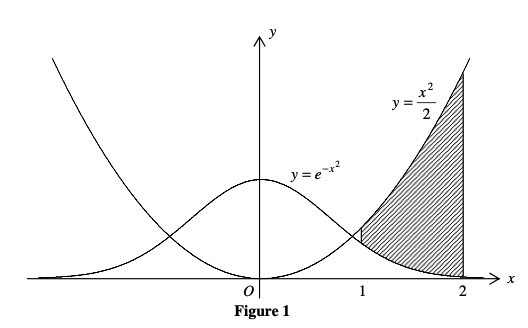
\includegraphics[width = .5\linewidth]{PPFigure1}
		\end{figure}
	\end{enumerate}

	\newpage

	\item \textbf{HKDSE Math M2 Practice Paper Q14}
	\begin{enumerate}
		\item[(a)]In Figure 3, the shaded region enclosed by the circle $x^2 + y^2 = 25$, the $x$-axis and the straight line $y = h$ (where $0 \leq h \leq 5$) is revolved about the $y$-axis. \\
		Show that the volume of the solid of revolution is $\left(25h - \displaystyle\frac{h^3}{3}\right)\pi$. \\(2 marks)
		\begin{figure}[H]
			\centering
			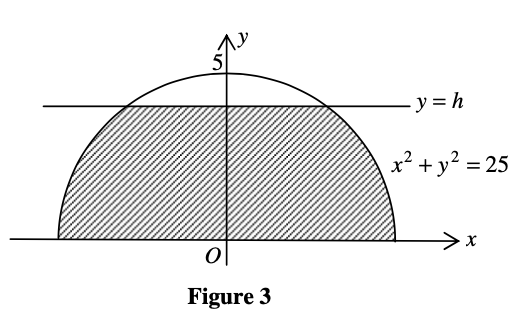
\includegraphics[width = .5\linewidth]{PPFigure3}
		\end{figure}		
		\item[(b)]In Figure 4, an empty coffee cup consists of two portions. The lower portion is in the shape of the solid described in (a) with height 4 cm. The upper portion is a frustum of a circular cone. The height of the frustum is 8 cm. The radius of the top of the cup is 6 cm. Hot coffee is poured into the cup to a depth $h$ cm at a rate of 8 cm$^3$s$^{-1}$, where $0 \leq h \leq 12$. Let $V$ cm$^3$ be the volume of coffee in the cup. 
		\begin{figure}[H]
			\centering
			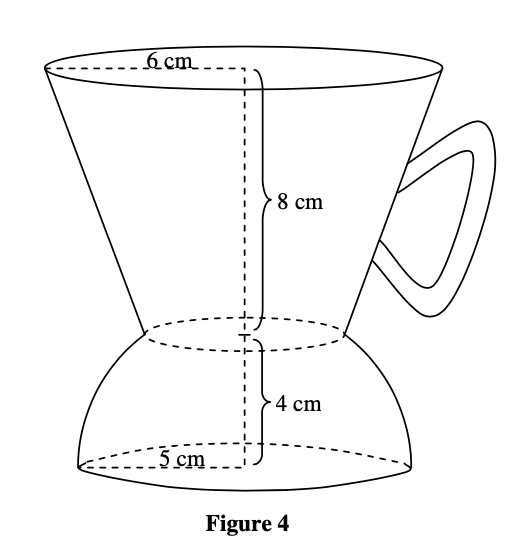
\includegraphics[width = .5\linewidth]{PPFigure4}
		\end{figure}
		\begin{enumerate}
			\item [(i)]Find the rate of increase of the depth of coffee when the depth is 3 cm.
			\item [(ii)]Show that $$V = \displaystyle\frac{164\pi}{3} + \frac{3\pi}{64}(h+4)^3$$ for $4\leq h \leq 12$. 
			\item [(iii)]After the cup is fully filled, suddenly it cracks at the bottom. The coffee leaks at a rate of 2 cm$^3$s$^{-1}$. Find the rate of decrease of the depth of coffee after 15 seconds of leaking, giving your answer correct to 3 significant figures.
		\end{enumerate}
		(11 marks)
	\end{enumerate}

	\newpage

	\item \textbf{HKDSE Math M2 2012 Q9}
	\begin{enumerate}
		\item [(a)]Using integration by parts, find $\int x\sin{x}\,dx$. 
		\item [(b)]Figure 4 shows the shaded region bounded by the curve $y = \sqrt{x\sin{x}}$ for $0 \leq x \leq \pi$ and the $x$-axis. Find the volume of the solid generated by revolving the region about the $x$-axis.
	\begin{figure}[H]
		\centering
		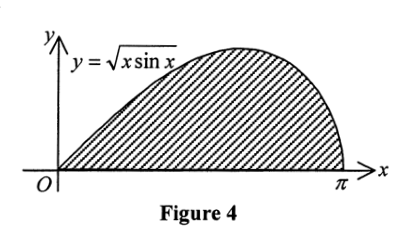
\includegraphics[width = .5\linewidth]{2012Figure4}
	\end{figure}
	\end{enumerate}
	(4 marks)

	\newpage

	\item \textbf{HKDSE Math M2 2012 Q14}\\
	Consider the curve $\Gamma : y = kx^p$, where $k>0$, $p > 0$. In Figure 7, the tangent to $\Gamma$ at $A(a, ka^{p})$ cuts the $x$-axis at $B(-a, 0)$, where $a>0$.
	\begin{figure}[H]
		\centering
		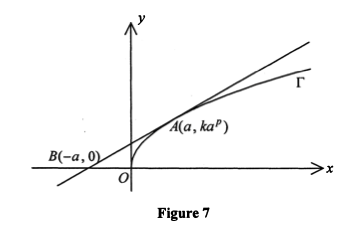
\includegraphics[width = .5\linewidth]{2012Figure7}
	\end{figure}
	\begin{enumerate}
		\item [(a)]Show that $\displaystyle p = \frac{1}{2}$. \\(3 marks)
		\item [(b)]Suppose that $a = 1$. As shown in Figure 8, the circle $C$, with radius 2 and centre on the $y$-axis, touches $\Gamma$ at point $A$.
		\begin{figure}[H]
			\centering
			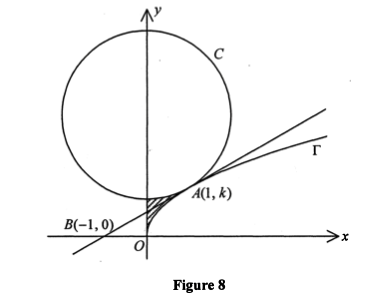
\includegraphics[width = .5\linewidth]{2012Figure8}
		\end{figure}
		\begin{enumerate}
			\item [(i)]Show that $\displaystyle k = \frac{2\sqrt{3}}{3}$. 
			\item [(ii)]Find the area of the shaded region bounded by $\Gamma$, $C$ and the $y$-axis.
		\end{enumerate}
		(9 marks)
	\end{enumerate}

	\item \textbf{HKDSE Math M2 2013 Q4}\\
	The slope at any point $(x,y)$ of a curve is given by $\displaystyle\frac{dy}{dx} = e^x - 1$. It is given that the curve passes through the point $(1,e)$. 
	\begin{enumerate}
		\item [(a)]Find the equation of the curve.
		\item [(b)]Find the equation of tangent to the curve at the point where the curve cuts the $y$-axis.
	\end{enumerate}
	(5 marks)

	\newpage

	\item \textbf{HKDSE Math M2 2013 Q6}\\
	Figure 1 shows the shaded region with boundaries $C : y = \displaystyle\frac{-x^2}{2} + 2x + 4$, $L_1 : y = 4$ and $L_2 : x = 5$. \\
	It is given that $C$ intersects $L_1$ at $(0,4)$ and $(4,4)$. 
	\begin{figure}[H]
		\centering
		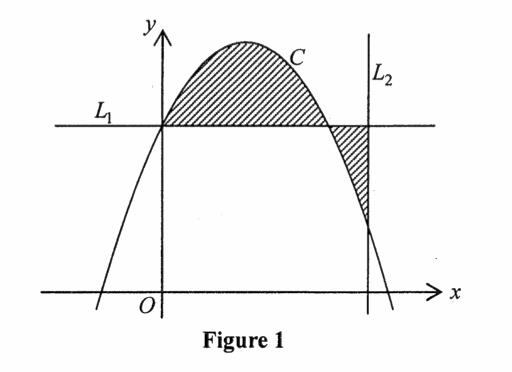
\includegraphics[width = .4\linewidth]{2013Figure1}
	\end{figure}
	\begin{enumerate}
		\item [(a)]Find the area of the shaded region.
		\item [(b)]Find the volume of solid of revolution when the shaded region is revolved about $L_1$.
	\end{enumerate}
	(6 marks)

	\item \textbf{HKDSE Math M2 2014 Q6}
	\begin{enumerate}
		\item [(a)]Find $\displaystyle\int xe^{-x}\,dx$. 
		\item [(b)]Figure 1 shows the shaded region bounded by the curve $y = xe^{-x}$ and the straight line $y = \displaystyle\frac{x}{e}$. \\
		Find the area of the shaded region.
		\begin{figure}[H]
			\centering
			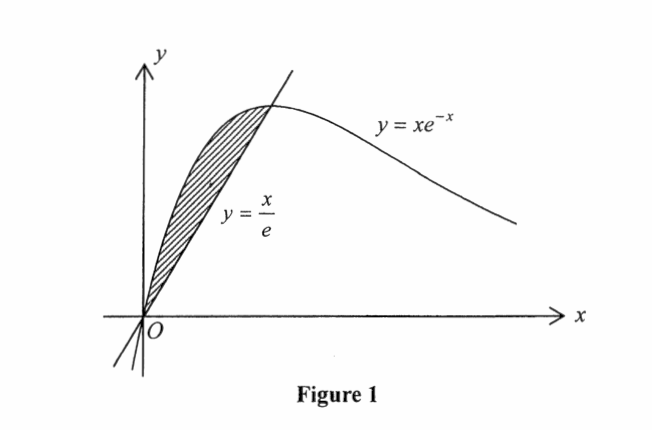
\includegraphics[width = .5\linewidth]{2014Figure1}
		\end{figure}
	\end{enumerate}
	(6 marks)

	\newpage

	\item \textbf{HKDSE Math M2 2014 Q13}
	\begin{enumerate}
		\item [(a)]Prove that $$1 - \cos{4\theta} - 2\cos{2\theta}\sin^2{2\theta} = 16\cos^2{\theta}\sin^4{\theta}.$$ \\(2 marks)
		\item [(b)]Show that $\displaystyle\int_{0}^{n\pi} \cos^2{x}\sin^4{x} \,dx = \displaystyle\frac{n\pi}{16}$, where $n$ is a positive integer.\\(4 marks)
		\item [(c)]Let $f(x)$ be a continuous function such that $f(k-x) = f(x)$, where $k$ is a constant. Show that $$\displaystyle\int_{0}^k xf(x)\, dx = \frac{k}{2} \int_{0}^k f(x) \,dx.$$
		(4 marks)
		\item [(d)]Figure 5 shows the shaded region bounded by curve $y = cos^2{x} \sin^4{x}$ and the $x$-axis, \\
		where $\pi \leq x \leq 2\pi$. Find the volume of the solid of revolution when the shaded region is revolved about the $y$-axis.\\
		(4 marks)
			\begin{figure}[H]
				\centering
				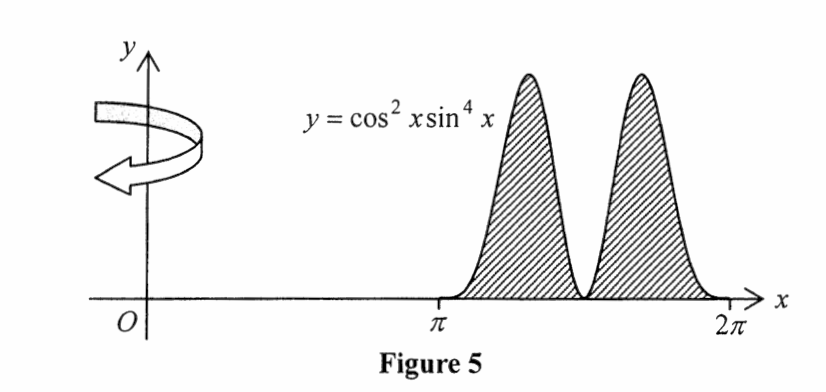
\includegraphics[width = .5\linewidth]{2014Figure5}
			\end{figure}
	\end{enumerate}

	\item \textbf{HKDSE Math M2 2015 Q4}
	\begin{enumerate}
		\item [(a)]Using integration by parts, find $\displaystyle\int x^2 \ln{x} \,dx $. 
		\item [(b)]At any point $(x,y)$ on the curve $\Gamma $, the slope of the tangent to $\Gamma$ is $9x^2 \ln{x}$. It is given that $\Gamma$ passes through the point $(1,4)$. Find the equation of $\Gamma$.  
	\end{enumerate}
	(7 marks)

	\newpage

	\item \textbf{HKDSE Math M2 2015 Q12}
	\begin{enumerate}
		\item [(a)]In the figure, the curve $\Gamma$ consists of curve $AB$, the line segments $BC$ and $CO$, where $O$ is the origin, $B$ lies in the first quadrat and $C$ lies on the $x$-axis. The equations of $AB$ and $BC$ are $x^2-4y+8 = 0$ and $3x+y-9=0$ respectively.
			\begin{figure}[H]
				\centering
				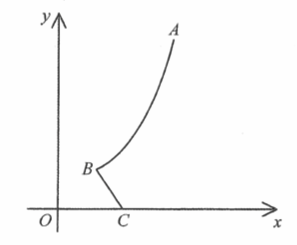
\includegraphics[width = .3\linewidth]{2015Figure1}
			\end{figure}
		\begin{enumerate}
			\item [(i)]Find the coordinates of $B$. 
			\item [(ii)]Let $h$ be the $y$-coordinate of $A$, where $h > 3$. A cup is formed by revolving $\Gamma$ about the $y$-axis.\\
			Prove that the capacity of the cup is $\pi(2h^2-8h+25)$.
		\end{enumerate}
		(7 marks)
		\item [(b)]A cup described in (a)(ii) is placed on a horizontal table. The radii of the base and the lip of the cup are 3 cm and 6 cm respectively.
		\begin{enumerate}
			\item [(i)]Find the capacity of the cup.
			\item [(ii)]Water is poured into the cup at a constant rate of $24\pi$ cm$^3$/s. Find the rate of change of the depth of water when the volume of water in the cup is $35\pi$ cm$^3$.
		\end{enumerate}
		(6 marks)
	\end{enumerate}

	\item \textbf{HKDSE Math M2 2016 Q7}
	\begin{enumerate}
		\item [(a)]Using integration by substitution, find $\displaystyle\int (1+\sqrt{t+1})^2 \,dt$. 
		\item [(b)]Consider the curve $\Gamma : y = 4x^2 - 4x$, where $1 \leq x \leq 4$. Let $R$ be the region bounded by $\Gamma$, the straight line $y=48$ and the two axes. Find the volume of the solid of revolution generated by revolving $R$ about the $y$-axis.
	\end{enumerate}
	(8 marks)
	
	\item \textbf{HKDSE Math M2 2016 Q9}\\
	Let $a$ and $b$ be constants. Define $f(x) = x^3 + ax^2 + bx + 5$ for all real numbers $x$. Denote the curve $y = f(x)$ by $C$. It is given that $P(-1,10)$ is a turning point of $C$.
	\begin{enumerate}
		\item [(a)]Find $a$ and $b$.\\(3 marks)
		\item [(b)]Is $P$ a maximum point of $C$? Explain your answer. \\(2 marks)
		\item [(c)]Find the minimum value(s) of $f(x)$. \\(2 marks)
		\item [(d)]Find the point(s) of inflexion of $C$. \\(2 marks)
		\item [(e)]Let $L$ be the tangent to $C$ at $P$. Find the area of the region bounded by $C$ and $L$. \\(4 marks)
	\end{enumerate}
	
	\item \textbf{HKDSE Math M2 2017 Q4}	
	\begin{enumerate}
		\item [(a)]Using integration by parts, find $\displaystyle\int x^2 e^{-x} \,dx$. 
		\item [(b)]Find the area of the region bounded by the graph of $y = x^2 e^{-x}$, the $x$-axis and the straight line $x = 6$.
	\end{enumerate}
	(6 marks)

	\newpage

	\item \textbf{HKDSE Math M2 2017 Q9}\\
	Define $f(x) = \displaystyle\frac{x^2 - 5x}{x + 4}$ for all $x \neq -4$. Denote the graph of $y = f(x)$ by $G$. 
	\begin{enumerate}
		\item [(a)]Find the asymptote(s) of $G$.  \\(3 marks)
		\item [(b)]Find $f'(x)$. \\(2 marks) 
		\item [(c)]Find the maximum point(s) and the minimum point(s) of $G$. \\(4 marks) 
		\item [(d)]Let $R$ be the region bounded by $G$ and the $x$-axis. Find the volume of the solid of revolution generated by revolving $R$ about the $x$-axis. \\(4 marks)
	\end{enumerate}

	\item \textbf{HKDSE Math M2 2018 Q4}
	\begin{enumerate}
		\item [(a)]Using integration by parts, find $\displaystyle\int u(5^u) \,du$. 
		\item [(b)]Define $f(x) = x(5^{2x})$ for all real numbers $x$. Find the area of the region bounded by the graph of $y = f(x)$, the straight line $x = 1$ and the $x$-axis.
	\end{enumerate}
	(6 marks)

	\item \textbf{HKDSE Math M2 2018 Q10}
	\begin{enumerate}
		\item [(a)] 
		\begin{enumerate}
			\item [(i)]Prove that $$\displaystyle \int \sin^4{x}\,dx = \frac{-\cos{x}\sin^3{x}}{4} + \frac{3}{4} \int \sin^2{x} \,dx.$$ 
			\item [(ii)] Evaluate $\displaystyle \int_{0}^{\pi} \sin^4{x}\,dx$.
		\end{enumerate}
		(5 marks)
		\item [(b)] 
		\begin{enumerate}
			\item [(i)]Let $f(x)$ be a continuous function such that $f(\beta - x)= f(x)$ for all real numbers $x$, where $\beta$ is a constant. Prove that $$\displaystyle\int_{0}^{\beta} x f(x) \,dx = \frac{\beta}{2} \int_{0}^{\beta } f(x) \,dx.$$
			\item [(ii)] Evaluate $\displaystyle \int_{0}^{\pi} x\sin^4{x}\,dx$.
		\end{enumerate}
		(5 marks)
	\item [(c)]Consider the curve $G : y = \displaystyle \sqrt{x}\sin^2{x}$, where $\pi \leq x \leq 2\pi $.
	Let $R$ be the region bounded by $G$ and the $x$-axis.
	Find the volume of the solid of revolution generated by revolving $R$ about the $x$-axis. \\(3 marks) 
	\end{enumerate}

	\item \textbf{HKDSE Math M2 2019 Q4}\\
	Define $\displaystyle g(x) = \frac{\ln{x}}{\sqrt{x}}$ for all $x \in (0,99)$. Denote the graph of $y = g(x) $ by $G$. 
	\begin{enumerate}
		\item [(a)]Prove that $G$ has only one maximum point. 
		\item [(b)]Let $R$ be the region bounded by $G$, the $x$-axis and the vertical line passing through the maximum point of $G$. Find the volume of the solid of revolution generated by revolving $R$ about the $x$-axis.
	\end{enumerate}
	(6 marks)

	\newpage

	\item \textbf{HKDSE Math M2 2019 Q9}\\
	Consider the curve $\Gamma : y = \displaystyle\frac{1}{3}\sqrt{12-x^2}$, where $0<x<2\sqrt{3}$. Denote the tangent of $\Gamma$ at $x = 3$ by $L$.  
	\begin{enumerate}
		\item [(a)]Find the equation of $L$. \\(3 marks)
		\item [(b)]Let $C$ be the curve $y = \sqrt{4-x^2}$, where $0<x<2$. It is given that $L$ is a tangent to $C$. Find 
		\begin{enumerate}
			\item [(i)]the point(s) of contact of $L$ and $C$;  
			\item [(ii)]the point(s) of intersection of $C$ and $\Gamma$;  
			\item [(iii)]the area of region bounded by $L$, $C$ and $\Gamma$.
		\end{enumerate}
		(9 marks)
	\end{enumerate}

	\item \textbf{HKDSE Math M2 2020 Q4}
	\begin{enumerate}
		\item [(a)]Find $\displaystyle \int \sin^2{\theta} \,d\theta$. 
		\item [(b)]Define $\displaystyle f(x) = 4x(1-x^2)^{\frac{1}{4}}$ for all $x \in [0,1]$. Denote the graph of $y = f(x) $ by $G$. \\
		Let $R$ be the region bounded by $G$ and the $x$-axis. \\
		Find the volume of the solid of revolution generated by revolving $R$ about the $x$-axis.
	\end{enumerate}
	(6 marks)

	\item \textbf{HKDSE Math M2 2020 Q7}\\
	Let $f(x)$ be a continuous function defined on $\mathbb{R}$. Denote the curve $y = f(x)$ by $\Gamma$. \\
	It is given that $\Gamma $ passes through the point $(1,2)$ and $f'(x) = -2x+8$ for all $x \in \mathbb{R}$. 
	\begin{enumerate}
		\item [(a)]Find the equation of $\Gamma$. 
		\item [(b)]Let L be a tangent to $\Gamma$ such that $L$ passes through the point $(5,14)$ and the slope of $L$ is negative. Denote the point of contact of $\Gamma$ and $L$ by $P$. Find 
		\begin{enumerate}
			\item [(i)]the coordinates of $P$, 
			\item [(ii)]the equation of the normal to $\Gamma $ at $P$.
		\end{enumerate}
	\end{enumerate}
	(8 marks)

	\item \textbf{HKDSE Math M2 2020 Q9}\\
	Let $\displaystyle f(x) = \frac{(x+4)^3}{(x-4)^2}$ for all real numbers $x \neq 4$. Denote the graph of $y = f(x)$ by $H$.
	\begin{enumerate}
		\item [(a)] Find the asymptote(s) of $H$. \\(3 marks)
		\item [(b)] Find $f''(x)$. \\(2 marks)
		\item [(c)] Someone claims that there are two turning points of $H$. Do you agree? Explain your answer. \\(2 marks)
		\item [(d)] Find the point(s) of inflexion of $H$. \\(2 marks)
		\item [(e)] Find the area of the region bounded by $H$, the $x$-axis and the $y$-axis. \\(3 marks)
	\end{enumerate}

	\item \textbf{HKDSE Math M2 2021 Q6}\\
	Consider the curve $\Gamma : y = e^{2x-6}$. Denote the normal to $\Gamma$ at the point $(3,1)$ by $L$. \\
	Let $c$ be the $x$-intercept of $L$. Find
	\begin{enumerate}
		\item [(a)]$c$;
		\item [(b)]the area of the region bounded by $L$, $\Gamma$ and the straight line $x=c$.
	\end{enumerate}
	(7 marks)

	\newpage

	\item \textbf{HKDSE Math M2 2021 Q7}
	\begin{enumerate}
		\item [(a)]Using integration by parts, find $\displaystyle\int (\ln{x})^2 \,dx$.
		\item [(b)] Consider the curve $\displaystyle C : y = \sqrt{x}\ln{(x^2+1)}$, where $x\geq 0$. Let $R$ be the region bounded by $C$, the straight line $x=1 $ and the $x$-axis. Find the volume of the solid of revolution generated by revolving R about the $x$-axis.
	\end{enumerate}
	(7 marks)

	\item \textbf{HKDSE Math M2 2022 Q6}
	\begin{enumerate}
		\item [(a)]Using integration by substitution, prove that $$\displaystyle \int \frac{1}{x^2+2x+5}\,dx = \frac{1}{2} \tan^{-1} \left(\frac{x+1}{2}\right) +\text{ constant.}$$
		\item [(b)]At any point $(x,y)$ on the curve $G$, the slope of the tangent to $G$ is $\displaystyle \frac{2x+1}{x^2+2x+5}$.\\
		Given that $G$ passes through the point $(-3, \ln{2})$, does $G$ pass through the point $\displaystyle \left(-1, \frac{-\pi}{8}\right)$? \\
		Explain your answer.
	\end{enumerate}
	(7 marks)

	\item \textbf{HKDSE Math M2 2022 Q6}
	\begin{enumerate}
		\item [(a)]Using integration by substitution, prove that $$\displaystyle \int \frac{1}{x^2+2x+5}\,dx = \frac{1}{2} \tan^{-1} \left(\frac{x+1}{2}\right) +\text{ constant.}$$
		\item [(b)]At any point $(x,y)$ on the curve $G$, the slope of the tangent to $G$ is $\displaystyle \frac{2x+1}{x^2+2x+5}$.\\
		Given that $G$ passes through the point $(-3, \ln{2})$, does $G$ pass through the point $\displaystyle \left(-1, \frac{-\pi}{8}\right)$? \\
		Explain your answer.
	\end{enumerate}
	(7 marks)

\end{enumerate}

\chapter{Matrices}
\begin{enumerate}
	\item \textbf{HKDSE Math M2 Sample Paper Q10}\\
	Let $0^{\circ} < \theta < 180^{\circ}$ and define $A = \begin{pmatrix}\cos{\theta}&-\sin{\theta}\\\sin{\theta}&\cos{\theta}\\\end{pmatrix}$. 
	\begin{enumerate}
		\item [(a)]Prove, by mathematical induction, that
		$$A^n = \begin{pmatrix}\cos{n\theta}&-\sin{n\theta}\\\sin{n\theta}&\cos{n\theta}\\\end{pmatrix}$$ for all positive integers $n$.
		\item [(b)]Solve $\sin{3\theta} + \sin{2\theta} + \sin{\theta} = 0$.
		\item [(c)]It is given that $A^3 + A^2 + A = \begin{pmatrix}a&0\\0&a\\\end{pmatrix}$.\\Find the value(s) of $a$. 
	\end{enumerate}
	(8 marks)

	\item \textbf{HKDSE Math M2 Sample Paper Q11}\\
	Let $A = \begin{pmatrix}
		2 & 0 & 0\\
		1 & 1 & 0\\
		1 & 0 & 1\\
	\end{pmatrix}$, $P = \begin{pmatrix}
		0 & 0 & 1\\
		0 & 1 & 1\\
		1 & 1 & 1\\
	\end{pmatrix}$ and $D = \begin{pmatrix}
		1 & 0 & 0\\
		0 & 1 & 0\\
		0 & 0 & 2\\
	\end{pmatrix}$.
	\begin{enumerate}
		\item [(a)]Let $I$ and $O$ be the $3\times3$ identity matrix and zero matrix respectively. 
		\begin{enumerate}
			\item [(i)]Prove that $$P^3 -2P^2 - P + I = O.$$
			\item [(ii)]Using the result of (i), or otherwise, find $P^{-1}$.
		\end{enumerate}
		(5 marks)
		\item [(b)]
		\begin{enumerate}
			\item [(i)]Prove that $$D = P^{-1}AP.$$ 
			\item [(ii)]Prove that $D$ and $A$ are non-singular. 
			\item [(iii)]Find $(D^{-1})^{100}$. \\
			Hence, or otherwise, find $(A^{-1})^{100}$.
		\end{enumerate}
		(7 marks)
	\end{enumerate}

	\item \textbf{HKDSE Math M2 Practice Paper Q5}
	\begin{enumerate}
		\item [(a)]It is given that $\cos{(x+1)} + \cos{(x-1)} = k\cos{x}$ for any real $x$. Find the value of $k$. 
		\item [(b)]Without using a calculator, find the value of $\begin{vmatrix}
			\cos{1} & \cos{2} & \cos{3}\\
			\cos{4} & \cos{5} & \cos{6}\\
			\cos{7} & \cos{8} & \cos{9}\\
		\end{vmatrix}$.
	\end{enumerate}
	(6 marks)

	\newpage

	\item \textbf{HKDSE Math M2 Practice Paper Q11}\\
	Let $A = \begin{pmatrix}
		\alpha + \beta & -\alpha\beta \\
		1 & 0 \\
	\end{pmatrix}$ where $\alpha$ and $\beta$ are distinct real numbers. Let $I$ be the $2\times2$ identity matrix.  
	\begin{enumerate}
		\item [(a)]Show that $$A^2 = (\alpha +\beta)A - \alpha\beta I.$$ \\(2 marks)
		\item [(b)]Using (a), or otherwise, show that $(A - \alpha I)^2 = (\beta - \alpha)(A - \alpha I)$ and $(A - \beta I)^2 = (\alpha - \beta)(A - \beta I)$. \\(3 marks)
		\item [(c)]Let $X = s(A-\alpha I)$ and $Y = t(A-\beta I)$ where $s$ and $t$ are real numbers. \\
		Suppose $A = X + Y$.
		\begin{enumerate}
			\item [(i)]Find $s$ and $t$ in terms of $\alpha$ and $\beta$.
			\item [(ii)]For any positive integer $n$, prove that
			$$X^n = \displaystyle\frac{\beta^n}{\beta - \alpha} (A - \alpha I)\text{ and }Y^n = \displaystyle\frac{\alpha^n}{\alpha - \beta}(A - \beta I).$$
			\item [(iii)]For any positive integer $n$, express $A^n$ in the form of $pA + qI$, where $p$ and $q$ are real numbers. 
			
			[Note: It is known that for any $2\times2 $ matrices $H$ and $K$, \\
			if $HK = KH = \begin{pmatrix}
				0&0\\0&0\\
			\end{pmatrix}$, then $(H+K)^n = H^n + K^n$ for any positive integer $n$.]
		\end{enumerate}
		(9 marks)
	\end{enumerate}

	\item \textbf{HKDSE Math M2 2012 Q11}
	\begin{enumerate}
		\item [(a)]Solve the equation \\$\begin{vmatrix}
			1-x & 4  \\ 
			2 & 3-x  \notag
		\end{vmatrix} = 0 $ --------------(*). \\(2 marks)
		\item [(b)]Let $x_1 ,\, x_2  $ $(x_1<x_2)$ be the roots of (*). Let $P = \begin{pmatrix}
			a&c\\b&1\\
		\end{pmatrix}$. It is given that \\
		$\begin{pmatrix}1&4\\2&3\\\end{pmatrix}\begin{pmatrix}a\\b\\\end{pmatrix} = x_1 \begin{pmatrix}a\\b\\\end{pmatrix}$, $\begin{pmatrix}1&4\\2&3\\\end{pmatrix}\begin{pmatrix}c\\1\\\end{pmatrix} = x_2 \begin{pmatrix}c\\1\\\end{pmatrix}$ and $|P| =1$,\\
		where $a$, $b$ and $c$ are constants.
		\begin{enumerate}
			\item [(i)]Find $P$.
			\item [(ii)]Evaluate $P^{-1}\begin{pmatrix}1&4\\2&3\\\end{pmatrix}P$.
			\item [(iii)]Using (b)(ii), evaluate $\begin{pmatrix}1&4\\2&3\\\end{pmatrix}^{12}$.
		\end{enumerate}
		(11 marks)
	\end{enumerate}

	\item \textbf{HKDSE Math M2 2013 Q8}\\
	Let $M$ be the matrix $\begin{pmatrix}
		1 & k & 0\\
		0 & 1 & 1\\
		k & 0 & 0\\
	\end{pmatrix}$, where $k \neq 0$. 
	\begin{enumerate}
		\item [(a)]Find $M^{-1}$. 
		\item [(b)]If $M\begin{pmatrix}
		x\\
		1\\
		z\\
	\end{pmatrix} = \begin{pmatrix}
		2\\
		2\\
		1\\
	\end{pmatrix}$, find the value of $k$.
	\end{enumerate}
	(5 marks)

	\newpage

	\item \textbf{HKDSE Math M2 2013 Q13}\\
	For any matrix $M = \begin{pmatrix}
		a&b\\c&d\\
	\end{pmatrix}$, define tr($M$) $= a + d$.\\
	Let $A$ and $B$ be $2 \times 2$ matrices such that $BAB^{-1} = \begin{pmatrix}
		1&0\\0&3\\
	\end{pmatrix}$. 
	\begin{enumerate}
		\item [(a)]
		\begin{enumerate}
			\item [(i)]For any matrix $N = \begin{pmatrix}
				e&f\\g&h\\
			\end{pmatrix}$, prove that tr(\textit{MN}) = tr(\textit{NM}).
			\item [(ii)]Show that $\text{tr}(A) = 4$. 
			\item [(iii)]Find the value of $|A|$.
		\end{enumerate}
		(6 marks)
		\item [(b)]Let $C = \begin{pmatrix}
			p&q\\r&s\\
		\end{pmatrix}$. It is given that $C \begin{pmatrix} x\\y\\ \end{pmatrix} = \lambda_1\begin{pmatrix} x\\y\\ \end{pmatrix}$ and $C \begin{pmatrix} x\\y\\ \end{pmatrix} = \lambda_2\begin{pmatrix} x\\y\\ \end{pmatrix}$ for some non-zero matrices $\begin{pmatrix} x\\y\\ \end{pmatrix}$ and distinct scalars $\lambda_1$ and $\lambda_2$. 
		\begin{enumerate}
			\item [(i)]Prove that $\begin{vmatrix}
				p - \lambda_1 & q \\ 
				r & s - \lambda_1   \notag
				\end{vmatrix} = 0$ and $\begin{vmatrix}
				p - \lambda_2 & q \\ 
				r & s - \lambda_2   \notag
				\end{vmatrix} = 0$. 
			\item [(ii)]Prove that $\lambda_1$ and $\lambda_2$ are the roots of the equation $$\lambda^2 - \text{tr}(C) \cdot \lambda + |C| = 0.$$
		\end{enumerate}
		(5 marks)
		\item [(c)]Find the two values of $\lambda$ such that $A\begin{pmatrix}
			x\\y\\
		\end{pmatrix} = \lambda \begin{pmatrix}
			x\\y\\
		\end{pmatrix}$ for some non-zero matrices $\begin{pmatrix}
			x\\y\\
		\end{pmatrix}$. \\(2 marks)
	\end{enumerate}

	\item \textbf{HKDSE Math M2 2014 Q7}\\
	Let $A = \begin{pmatrix}
		1&0&1\\
		0&2&0\\
		1&0&1\\
	\end{pmatrix}$.
	\begin{enumerate}
		\item [(a)]Prove, by mathematical induction, that for all positive integers $n$, $$A^{n+1} = 2^nA.$$ 
		\item [(b)]Using the result of (a), Willy proceeds in the following way:\\
			$A^2 = 2A$\\
			$A^2 A^{-1}= 2AA^{-1}$\\
			$A = 2I$\\
			Explain why Willy arrives at a wrong conclusion.
	\end{enumerate}
	(7 marks)

	\item \textbf{HKDSE Math M2 2014 Q12}\\
	Let $M = \begin{pmatrix}
		k-1&k\\
		1  &0\\
	\end{pmatrix}$ and $A = \begin{pmatrix}
		1&p\\
		-1&1\\
	\end{pmatrix}$, where $k$ and $p$ are real numbers and $p \neq -1$. 
	\begin{enumerate}
		\item [(a)]
		\begin{enumerate}
			\item [(i)]Find $A^{-1}$ in terms of $p$. 
			\item [(ii)]Show that $$A^{-1}MA =  
			\begin{pmatrix}
				-1&k-p\\
				0 &k\\
			\end{pmatrix}$$. 
			\item [(iii)]Suppose $p = k$. Using (ii), find $M^n$ in terms of $k$ and $n$, where $n$ is a positive integer.
		\end{enumerate}
		(8 marks)
		\item [(b)]A sequence is defined by $x_1 = 0$, $x_2 = 1$ and $x_n = x_{n-1} + 2x_{n-2}$ for $n = 3,4,5,\cdots$. \\
			It is known that this sequence can be expressed in the matrix form $\begin{pmatrix} x_n\\x_{n-1} \end{pmatrix} = \begin{pmatrix} 1&2\\1&0\\ \end{pmatrix}\begin{pmatrix} x_{n-1}\\x_{n-2} \end{pmatrix}$.\\
			Using the result of (a)(iii), express $x_n$ in terms of $n$. \\(3 marks)
	\end{enumerate}

	\newpage

	\item \textbf{HKDSE Math M2 2015 Q6}
	\begin{enumerate}
		\item [(a)]Let $M$ be a $3 \times 3$ real matrix such that $M^T = -M$, where $M^T$ is the transpose of $M$.\\
		Prove that $|M| = 0$.
		\item [(b)]Let $A = \begin{pmatrix}
			-1&a&b\\
			-a&-1&-8\\
			-b&8&-1\\
		\end{pmatrix}$, where $a$ and $b$ are real numbers. Denote the $3 \times 3$ identity matrix by $I$.
		\begin{enumerate}
			\item [(i)]Using (a), or otherwise, prove that $|A+I| = 0$. 
			\item [(ii)]Someone claims that $A^3 + I$ is a singular matrix. Do you agree? Explain your answer.
		\end{enumerate}
	\end{enumerate}
	(6 marks)

	\item \textbf{HKDSE Math M2 2015 Q11}
	\begin{enumerate}
		\item [(a)]Let $\lambda$ and $\mu$ be real numbers such that $\mu - \lambda \neq 2$. Denote the $2 \times 2$ identity matrix by $I$.\\Define $\displaystyle A = \frac{1}{\lambda - \mu + 2} (I - \mu I + M)$ and $\displaystyle B = \frac{1}{\lambda - \mu + 2} (I +\lambda  I - M)$, \\where $M = \begin{pmatrix}
			\lambda & 1 \\ \lambda - \mu + 1 & \mu \\
		\end{pmatrix}$. 
		\begin{enumerate}
			\item [(i)]Evaluate $AB$, $BA$ and $A+B$. 
			\item [(ii)]Prove that $A^2 = A$ and $B^2 = B$. 
			\item [(iii)]Prove that $$M^n = (\lambda + 1)^nA + (\mu -1)^n B$$ for all positive integers $n$.
		\end{enumerate}
		(8 marks)
		\item [(b)]Using (a), or otherwise, evaluate $\begin{pmatrix}
			4&2\\0&6\\
		\end{pmatrix}^{315}$. \\(4 marks)
	\end{enumerate}

	\item \textbf{HKDSE Math M2 2016 Q8}\\
	Let $n$ be a positive integer.
	\begin{enumerate}
		\item [(a)]Define $A = 
		\begin{pmatrix}
			1&0\\1&1\\
		\end{pmatrix}$. Evaluate 
		\begin{enumerate}
			\item [(i)]$A^2$, 
			\item [(ii)]$A^n$,
			\item [(iii)]$(A^{-1})^n$.
		\end{enumerate}
		\item [(b)]Evaluate
		\begin{enumerate}
			\item [(i)]$\displaystyle\sum_{k=0}^{n-1} 2^k$,
			\item [(ii)]$\begin{pmatrix}
				1&0\\1&2\\
			\end{pmatrix} ^n$.
		\end{enumerate}
	\end{enumerate}
	(8 marks)
	
	\newpage

	\item \textbf{HKDSE Math M2 2017 Q12}\\
	Let $A = \begin{pmatrix}
		3 & 1\\
		0 & 3\\
	\end{pmatrix}$. Denote the $2 \times 2$ identity matrix by $I$.
	\begin{enumerate}
		\item [(a)]Using mathematical induction, prove that $$A^n = 3^nI + 3^{n-1}n\begin{pmatrix}
			0&1\\0&0\\
			\end{pmatrix}$$ for all positive integers $n$. \\(4 marks)

		\item [(b)]Let $B = \begin{pmatrix}
			5 & 1\\
			-4 & 1\\
			\end{pmatrix}$. 
		\begin{enumerate}
			\item [(i)]Define $P = \begin{pmatrix}
			-1 & 0\\
			2 & -1\\
			\end{pmatrix}$. Evaluate $P^{-1}BP$.  
			\item [(ii)]Prove that $$B^n = 3^nI + 3^{n-1}n\begin{pmatrix}
			2&1\\-4&-2\\
			\end{pmatrix}$$ for any positive integer $n$.
			\item [(iii)]Does there exist a positive integer $m$ such that $|A^m - B^m| = 4m^2$ ? Explain your answer.
		\end{enumerate}
		(8 marks)
	\end{enumerate}	

	\item \textbf{HKDSE Math M2 2018 Q7}\\
	Let $M = 
		\begin{pmatrix}
		7 &3 \\
		-1&5\\
		\end{pmatrix}$. Let $X = 
		\begin{pmatrix}
		a &6a \\
		b&c\\
		\end{pmatrix}$ be a non-zero real matrix such that $MX = XM$. 
	\begin{enumerate}
		\item[(a)]Express $b$ and $c$ in  terms of $a$. 
		\item[(b)]Prove that $X$ is a non-singular matrix.
		\item[(c)]Denote the transpose of $X$ by $X^T$. Express $(X^T)^{-1}$ in terms of $a$.
	\end{enumerate}
	(8 marks)

	\item \textbf{HKDSE Math M2 2019 Q11}\\
	Let $M = \begin{pmatrix}
		2 &7 \\
		-1&-6\\
	\end{pmatrix}$. Denote the $2 \times2$ identity matrix by $I$. 
	\begin{enumerate}
		\item[(a)]Find a pair of real numbers $a$ and $b$ such that $M^2 = aM + bI$. \\(3 marks) 
		\item[(b)]
		Prove that $$6M^n = (1-(-5)^n)M+(5+(-5)^n)I)$$ for all positive integers $n$. \\(4 marks)
		\item[(c)]Does there exist a pair of $2\times2$ real matrices $A$ and $B$ such that $(M^n)^{-1} = A +\displaystyle \frac{1}{(-5)^n}B$ for all positive integers $n$? Explain your answer. \\(5 marks)
	\end{enumerate}

	\item \textbf{HKDSE Math M2 2020 Q8}\\
	Define $P = \begin{pmatrix}
				-5&-2\\
				15&6\\
				\end{pmatrix}$ and $Q = 
				\begin{pmatrix}
				1&0\\
				0&0\\
				\end{pmatrix}$. Let $M = 
				\begin{pmatrix}
				1&a\\
				b&c\\
			\end{pmatrix}$ such that $|M| = 1$ and $PM = MQ$, \\
	where $a$, $b$ and $c$ are real numbers.
	\begin{enumerate}
		\item [(a)] Find $a,b$ and $c$. 
		\item [(b)] Define $R = 
				\begin{pmatrix}
				6&2\\
				-15&-5\\
				\end{pmatrix}$. 
		\begin{enumerate}
			\item [(i)]Evaluate $M^{-1}RM$. 
			\item [(ii)]Using the result of (b)(i), prove that $(\alpha P + \beta R)^{99} = \alpha^{99}P+\beta ^{99}R$ for any real numbers $\alpha$ and $\beta$. 
		\end{enumerate} 
	\end{enumerate}
	(8 marks)

	\newpage

	\item \textbf{HKDSE Math M2 2021 Q11}\\
	Define $P = \begin{pmatrix}
		\sin{\theta}&\cos{\theta}\\
		-\cos{\theta}&\sin{\theta}\\
		\end{pmatrix}$, where $\displaystyle \frac{\pi}{2} < \theta < \pi$.
	\begin{enumerate}
		\item [(a)] Let $A = 
			\begin{pmatrix}
			\alpha&\beta\\
			\beta&-\alpha\\
			\end{pmatrix}$, where $\alpha, \beta \in \mathbb{R}$.\\
			Prove that $$PAP^{-1} = \begin{pmatrix}
			-\alpha \cos{2\theta}+\beta \sin{2\theta} &-\beta\cos{2\theta}-\alpha \sin{2\theta}\\
			-\beta\cos{2\theta}-\alpha\sin{2\theta}&\alpha\cos{2\theta}-\beta \sin{2\theta}\\
			\end{pmatrix}.$$ \\(3 marks)
		\item[(b)]Let $B = \begin{pmatrix}
			1&\sqrt{3}\\
			\sqrt{3}&-1\\
			\end{pmatrix}$.
		\begin{enumerate}
			\item [(i)] Find $\theta$ such that $PBP^{-1} = \begin{pmatrix}
				\lambda&0\\
				0&\mu\\
				\end{pmatrix}$, where $\lambda$, $\mu \in \mathbb{R}$.
			\item [(ii)]Using the result of (b)(i), prove that $$B^n = 2^{n-2} \begin{pmatrix}
				(-1)^n+3&\sqrt{3}(-1)^{n+1} + \sqrt{3}\\
				\sqrt{3}(-1)^{n+1}+\sqrt{3}&3(-1)^n+1\\
				\end{pmatrix}$$
				for any positive integer $n$.
			\item [(iii)] Evaluate $(B^{-1})^{555}$. 
		\end{enumerate}
		(9 marks)
	\end{enumerate}

	\item \textbf{HKDSE Math M2 2022 Q11}
	\begin{enumerate}
		\item [(a)] Let $n$ be a positive integer. Denote the $2\times2$ identify matrix by $I$. 
		\begin{enumerate}
			\item [(i)] Let $A$ be a $2\times2$ matrix. Simplify $(I - A)(I + A + A^2 + \cdots + A^n)$.
			\item [(ii)]Let $A = 
				\begin{pmatrix}
				\cos{\theta}&-\sin{\theta}\\
				\sin{\theta}&\cos{\theta}\\
				\end{pmatrix} \text{, 
				where } \theta \text{ is not a multiple of } 2\pi$.\\
				It is given that $A^n = 
				\begin{pmatrix}
				\cos{n\theta}&-\sin{n\theta}\\
				\sin{n\theta}&\cos{n\theta}\\
				\end{pmatrix}$. 
			\begin{enumerate}
				\item [(1)] Prove that $$\displaystyle(I - A) ^{-1} = \frac{1}{2\sin{\displaystyle\frac{\theta}{2}}} 
					\begin{pmatrix}
						\sin{\displaystyle\frac{\theta}{2}}&-\cos{\displaystyle\frac{\theta}{2}}\\
						\cos{\displaystyle\frac{\theta}{2}}&\sin{\displaystyle\frac{\theta}{2}}\\
					\end{pmatrix}$$.
				\item[(2)] Using the result of (a)(i) and (a)(ii)(1), prove that $$I+A+A^2+\cdots+A^n = \displaystyle\frac{\sin{\displaystyle\frac{(n+1)\theta}{2}}}{\sin{\displaystyle\frac{\theta}{2}}}
					\begin{pmatrix}
						\cos{\displaystyle\frac{n\theta}{2}}&-\sin{\displaystyle\frac{n\theta}{2}}\\
						\sin{\displaystyle\frac{n\theta}{2}}&\cos{\displaystyle\frac{n\theta}{2}}\\
					\end{pmatrix}.$$
			\end{enumerate}
		\end{enumerate}
		(7 marks)
		\item[(b)]Using (a)(ii), evaluate
		\begin{enumerate}
			\item [(i)]$\cos{\displaystyle\frac{5\pi}{18}}+\cos{\displaystyle\frac{5\pi}{9}}+\cos{\displaystyle\frac{5\pi}{6}}+\cdots+\cos{25\pi}$ ; 
			\item [(ii)]$\cos^2{\displaystyle\frac{\pi}{7}}+\cos^2{\displaystyle\frac{2\pi}{7}}+\cos^2{\displaystyle\frac{3\pi}{7}}+\cdots+\cos^2{7\pi}$. 
		\end{enumerate}
	(6 marks)
	\end{enumerate}

	\item \textbf{HKDSE Math M2 2023 Q5}\\
	Let $A$ be $2\times2$ real matrix such that $A^2 + A + I = 0$, where $I$ is the $2\times2$ identity matrix. 
	\begin{enumerate}
		\item [(a)]Prove that $A^3 = I$.
		\item [(b)]Prove that $A$ is non-singular.
		\item [(c)]Someone claims that $\left(A^{1000} + (A^{-1})^{2000}\right)^{-1}$ can be expressed in the form of $\alpha I + \beta A$, where $\alpha$ and $\beta$ are real numbers. Is the claim correct? Explain your answer.
	\end{enumerate}
	(7 marks)

\end{enumerate}

\chapter{System of Linear Equations}
\begin{enumerate}
	\item \textbf{HKDSE Math M2 Sample Paper Q7}\\
	Solve the system of linear equations
	$$\left\{\begin{matrix}
		x & + & 7y & - & 6z & = & -4\\
		3x & - & 4y & + & 7z & = & 13\\
		4x & + & 3y & + & z & = & 9\\
	\end{matrix}\right..$$ \\(5 marks)

	\item \textbf{HKDSE Math M2 Practice Paper Q2}\\
	Consider the following system of linear equation in $x$, $y$, $z$
	$$\left\{\begin{matrix}
		x & - & 7y & + & 7z & = & 0\\
		x & - & ky & + & 3z & = & 0\\
		2x & + & y & + & kz & = & 0\\
	\end{matrix}\right.\text{ , where }k\text{ is a real number.}$$
	If the system has non-trival solutions, find the two possible values of $k$. \\(4 marks)

	\item \textbf{HKDSE Math M2 2012 Q8}
	\begin{enumerate}
		\item [(a)]Solve the following system of linear equations:
		$$\left\{\begin{matrix}
			x & + & y & + & z & = & 0\\
			2x & - & y & + & 5z & = & 6\\
		\end{matrix}\right.$$
		\item [(b)]Using (a), or otherwise, solve the following system of linear equations: 
		$$\left\{\begin{matrix}
			x & + & y & + & z & = & 0\\
			2x & - & y & + & 5z & = & 6\\
			x & - & y & + & \lambda z & = & 4\\
		\end{matrix}\right.\text{ , where }\lambda\text{ is a constant.}$$ 
	\end{enumerate}
	(5 marks)

	\item \textbf{HKDSE Math M2 2013 Q9}\\
	Consider the following system of linear equations in $x$, $y$ and $z$
		$$(E)  \left\{\begin{matrix}
		x & - & ay & + & z & = & 2\\
		2x & + & (1-2a)y & + & (2-b)z  & =  & a+4\\
		3x & + & (1-3a)y & + & (3-ab)z & = & 4\\
		\end{matrix}\right.,$$where $a$ and $b$ are real numbers. \\
		It is given that $(E)$ has infinitely many solutions.
	\begin{enumerate}
		\item [(a)]Find the values of $a$ and $b$.
		\item [(b)]Solve $(E)$.
	\end{enumerate}
	(5 marks)

	\newpage
	
	\item \textbf{HKDSE Math M2 2014 Q9}
	\begin{enumerate}
		\item [(a)]Solve the system of linear equations $\left\{
		\begin{matrix}
			x & + & y & + & z & = & 100\\
			x & + & 6y& + &10z& = & 200\\
		\end{matrix}\right.$
		\item [(b)]In a store, the prices of each of small, medium and large marbles are \$0.5, \$3 and \$5 respectively. Aubrey plans to spend all \$100 for exactly 100 marbles, which include $m$ small marbles, $n$ medium marbles and $k$ large marbles.\\
		Aubrey claims that there is only one set of combination of $m$, $n$ and $k$. Do you agree? Explain your answer.
	\end{enumerate}
	(6 marks)	

	\item \textbf{HKDSE Math M2 2015 Q5}\\
	Solve the following systems of linear equations in real variables $x$, $y$, $z$:
	\begin{enumerate}
		\item [(a)]$\left\{
			\begin{matrix}
				x&+&y&+&z&=&2\\
				2x&+&3y&-&3z&=&4\\
			\end{matrix}\right.$;
		\item [(b)]$\left\{
			\begin{matrix}
				x&+&y&+&z&=&2\\
				2x&+&3y&-&3z&=&4\\
				3x&+&2y&+&kz&=&6\\
			\end{matrix}\right.$, where $k$ is a real constant.
	\end{enumerate}
	(6 marks)

	\item \textbf{HKDSE Math M2 2016 Q11}
	\begin{enumerate}
		\item [(a)]Consider the system of linear equations in real variables $x$, $y$, $z$
		$$(E) : \left\{\begin{matrix}
		x &+&     y&-&      z&=&3  \\
		4x&+&    6y&+&     az&=&b  \\
		5x&+&(1-a)y&+&(3a-1)z&=&b-1\\
		\end{matrix}\right.\text{, where } a\text{ and } b\text{ are real numbers.}$$
		\begin{enumerate}
			\item [(i)]Assume that $(E)$ has a unique solution.
			\begin{enumerate}
				\item [(1)]Prove that $a\neq -2$ and $a \neq -12$.
				\item [(2)]Solve $(E)$. 
			\end{enumerate}
			\item [(ii)]Assume that $a = -2$ and $(E)$ is consistent.
			\begin{enumerate}
				\item [(1)]Find $b$. 
				\item [(2)]Solve $(E)$.
			\end{enumerate}
		\end{enumerate}
		(9 marks)
		\item [(b)] Is there a real solution of the system of linear equations
		$$\left\{\begin{matrix}
		x&+&y&-&z&=&3\\
		2x&+&3y&-&z&=&7\\
		5x&+&3y&-&7z&=&13\\
		\end{matrix}\right.$$
		satisfying $x^2+y^2-6z^2 > 14$? Explain your answer. \\(3 marks)
	\end{enumerate}

	\item \textbf{HKDSE Math M2 2017 Q5}\\
	Consider the following system of linear equations in real variables $x$, $y$, $z$
		$$(E) : \left\{\begin{matrix}
		x&  +&2y&  -&z& = &11  \\
		3x& +&8y&  -&11z& = & 49 \\
		2x& +&3y&  +&hz& = & k \\
		\end{matrix}\right.\text{, where } h,k \in \mathbb{R}.$$ 
	\begin{enumerate}
		\item [(a)] Assume that $(E)$ has a unique solution.
		\begin{enumerate}
			\item [(i)]Find the range of values of $h$.
			\item [(ii)]Express $z$ in terms of $h$ and $k$.
		\end{enumerate}
		\item [(b)]Assume that $(E)$ has infinitely many solutions. Solve $(E)$.
	\end{enumerate}
	(6 marks)

	\newpage
	
	\item \textbf{HKDSE Math M2 2018 Q11}
	\begin{enumerate}
		\item [(a)]Consider the system of linear equations in real variables $x$, $y$, $z$
		$$(E) : \left\{\begin{matrix}
		x&  +&ay&  +&4(a+1)z& = &18  \\
		2x& +&(a-1)y&  +&2(a-1)z& = & 20 \\
		x&  -&y&  -&12z& = & b \\
		\end{matrix}\right.\text{, where }a,b \in \mathbb{R}. $$
		\begin{enumerate}
			\item [(i)]Assume that $(E)$ has a unique solution.
			\begin{enumerate}
				\item [(1)]Find the range of values of $a$. 
				\item [(2)]Solve $(E)$. 
			\end{enumerate}			
			\item [(ii)]Assume that $a = 3 $ and $(E)$ is consistent.
			\begin{enumerate}
				\item [(1)]Find $b$. 
				\item [(2)]Solve $(E)$.
			\end{enumerate}
		\end{enumerate}
		(9 marks)
		\item [(b)]Consider the system of linear equations in real variables $x$, $y$, $z$
		$$(F) : \left\{\begin{matrix}
		x&  +&	3y&	+&	16z&	=& 18  \\
		x& 	+&	y&	+&	2z&		=& 20 \\
		x&  -&	y&  -&	12z&	=& s \\
		2x& -&	5y& -&	45z&	=& t \\
		\end{matrix}\right.\text{, where }s,t \in \mathbb{R}.$$
		Assume that $(F)$ is consistent. Find $s$ and $t$. \\(3 marks)
	\end{enumerate}

	\item \textbf{HKDSE Math M2 2019 Q6}\\
	Consider the system of linear equations in real variables $x$, $y$, $z$
	$$(E):\left\{\begin{matrix}
		 x&  -&2y&  -&2z& = &\beta  \\
		5x&  +&\alpha y&  +&\alpha z& = & 5\beta \\
	7x&  +&(\alpha - 3)y&  +&(2\alpha+1)z& = & 8\beta \\
		\end{matrix}\right.\text{, where }\alpha, \beta \in \mathbb{R}.$$
	\begin{enumerate}
		\item [(a)]Assume that $(E)$ has a unique solution.
		\begin{enumerate}
			\item [(i)]Find the range of values of $\alpha$. 
			\item [(ii)]Express $y$ in terms of $\alpha$ and $\beta$. 
		\end{enumerate}
		\item [(b)]Assume that $\alpha = -4$ . If  $(E)$ is inconsistent, find the range of values of $\beta$.
	\end{enumerate}
	(7 marks)

	\item \textbf{HKDSE Math M2 2020 Q11}
	\begin{enumerate}
		\item [(a)] Consider the system of linear equations in real variables $x$, $y$, $z$
		$$(E):\left\{\begin{matrix}
			x&  -& y& -&2z& = & 1  \\
			x&  -&2y& +&hz& = & k \\
			4x& +&hy& -&7z& = & 7 \\
		\end{matrix}\right. \text{, where }h,k \in \mathbb{R}.$$
		\begin{enumerate}
			\item [(i)]Assume that $(E)$ has a unique solution.
			\begin{enumerate}
				\item [(1)]Prove that $h \neq -3$. 
				\item [(2)]Solve $(E)$.
			\end{enumerate}
			\item [(ii)]Assume that $h = -3$ and $(E)$ is consistent.
			\begin{enumerate}
				\item [(1)]Prove that $k = -2$. 
				\item [(2)]Solve $(E)$. 
			\end{enumerate}
		\end{enumerate}
		(9 marks)
		\item[(b)]Consider the system of linear equations in real variables $x$, $y$, $z$
		$$(F):\left\{\begin{matrix}
		x&  -&y&  -&2z& = &1  \\
		x&  -&2y&  +&hz& = & -2 \\
		4x&  +&hy&  -&7z& = & 7 \\
		\end{matrix}\right. \text{, where }h \in \mathbb{R}.$$
		Someone claims that there are at least two values of $h$ such that $(F)$ has a real solution $(x,y,z)$ satisfying $3x^2+4y^2-7z^2=1$. Do you agree? Explain your answer. \\(4 marks)
	\end{enumerate}
	
	\newpage
	
	\item \textbf{HKDSE Math M2 2021 Q8}\\
	Consider the system of linear equations in real variables $x$, $y$, $z$
		$$(E) : \left\{\begin{matrix}
		x&  +&(d-1)y&  +&(d+3)z& = &4-d  \\
		2x&  +&(d+2)y&  -&z& = & 2d-5 \\
		3x&  +&(d+4)y&  +&5z& = & 2 \\
		\end{matrix}\right. \text{,  where } d \in \mathbb{R} .$$
		It is given that $(E)$ has infinitely many solutions.
	\begin{enumerate}
		\item [(a)] Find $d$. Hence, solve $(E)$.
		\item [(b)] Someone claims that $(E)$ has a real solution $(x,y,z)$ satisfying $xy + 2xz = 3$. Is the claim correct? \\
		Explain your answer. 
	\end{enumerate}
	(8 marks)

	\item \textbf{HKDSE Math M2 2022 Q8}\\
	Consider the system of linear equations in real variables $x$, $y$ and $z$
		$$(E) : \left\{\begin{matrix}
		ax&  +&2y&  -& z& = &4k  \\
		-x&  +&ay&  +&2z& = &4   \\
		2x&  -& y&  +&az& = &k^2 \\
		\end{matrix}\right. , \text{where } a,k \in \mathbb{R}$$
	\begin{enumerate}
		\item [(a)] Assume that $(E)$ has a unique solution. Express $y$ in terms of $a$ and $k$.
		\item [(b)] Assume that $(E)$ has infinitely many solutions. Solve $(E)$. 
	\end{enumerate}
	(7 marks)


	\item \textbf{HKDSE Math M2 2023 Q11}
	\begin{enumerate}
		\item [(a)] Consider the system of linear equations in real variables $x$, $y$, $z$
		$$(E) : \left\{\begin{matrix}
		x&	+&	ay&		+&	(a+1)z&		=&	2  \\
		x&	+&	(a+4)y&	+&	(2a+4)z&	=&	b+1 \\
		2x&	+&	3y&		+&	5z&			=&	b \\
		\end{matrix}\right. \text{,  where } a, b \in \mathbb{R} .$$
		\begin{enumerate}
			\item [(i)] Assume that $(E)$ has a unique solution. Find the range of values of $a$.
			\item [(ii)] Assume that $a = 1$. If $(E)$ is consistent, find $b$.
			\item [(iii)] Assume that $a \neq 1$ and $(E)$ is incnsistent. Find the range of values of $b$.
		\end{enumerate}
		(7 marks)
		\item [(b)] Consider the system of linear equations in real variables $x$, $y$, $z$
		$$(F) : \left\{\begin{matrix}
		x&	+&	2y&	+&	3z&	=&	2  \\
		x&	+&	6y&	+&	8z&	=&	s+1 \\
		2x&	+&	3y&	+&	5z&	=&	s \\
		\end{matrix}\right. \text{,  where } s \in \mathbb{R} .$$
		Does there exist a pair of real constants $m$ and $n$ (independent of $s$) such that for every $s\in\mathbb{R}$, $(F)$ has a real solution $(x,y,z)$ satisfying $mx + ny + z = -2$? Explain your answer. \\(6 marks) 
	\end{enumerate}

\end{enumerate}

\chapter{Vectors}
\begin{enumerate}
	\item \textbf{HKDSE Math M2 Sample Paper Q9}\\
	Let $\overrightarrow{OA} = 4\textbf{i} +3 \textbf{j}$, $\overrightarrow{OB} = 3 \textbf{j} +\textbf {k}$ and $\overrightarrow{OC} = 3\textbf{i} + \textbf{j} +5\textbf {k}$. Figure 2 shows the parallelepiped $OADBECFG$ formed by $\overrightarrow{OA}$, $\overrightarrow{OB}$ and $\overrightarrow{OC}$. 
	\begin{figure}[H]
		\centering
		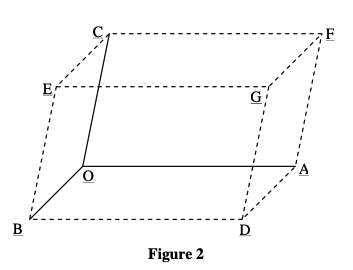
\includegraphics[width = .4\linewidth]{SPFigure2}
	\end{figure}
	\begin{enumerate}
		\item [(a)]Find the area of the parallelogram $OADB$.  
		\item [(b)]Find the volume of the parallelepiped $OADBECFG$.
		\item [(c)]If $C'$ is a point different from $C$ such that the volume of the parallelepiped formed by $\overrightarrow{OA}$, $\overrightarrow{OB}$ and $\overrightarrow{OC'}$ is the same as that of $OADBECFG$, find a possible vector of $\overrightarrow{OC'}$.
	\end{enumerate}
	(6 marks)

	\newpage
	
	\item \textbf{HKDSE Math M2 Sample Paper Q14}\\
	In Figure 3, $\triangle ABC$ is an acute-angled triangle, where $O$ and $H$ are the circumcentre and orthocentre respectively. Let $\overrightarrow{OA} = \textbf{a}$, $\overrightarrow{OB} = \textbf{b}$, $\overrightarrow{OC} = \textbf{c}$ and $\overrightarrow{OH} = \textbf{h}$.
	\begin{figure}[H]
		\centering
		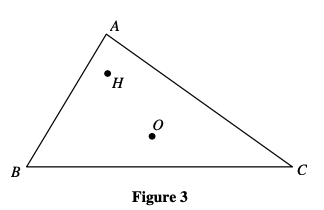
\includegraphics[width = .4\linewidth]{SPFigure3}
	\end{figure}
	\begin{enumerate}
		\item [(a)]Show that $$(\textbf{h} - \textbf{a})//(\textbf{b}+\textbf{c}).$$ \\(3 marks)
		\item [(b)]Let $\textbf{h} - \textbf{a} = t(\textbf{b}+\textbf{c})$, where $t$ is a non-zero constant.\\
		Show that 
		\begin{enumerate}
			\item [(i)]$t(\textbf{b}+\textbf{c}) + \textbf{a} - \textbf{b} = s(\textbf{c}+\textbf{a})$ for some scalar $s$, 
			\item [(ii)]$(t-1)(\textbf{b}-\textbf{a})\cdot (\textbf{c}-\textbf{a}) = 0$.
		\end{enumerate}
		(5 marks)
		\item[(c)]Express $\textbf{h}$ in terms of $\textbf{a}$, $\textbf{b}$ and $\textbf{c}$. \\(2 marks)
	\end{enumerate}

	\item \textbf{HKDSE Math M2 Practice Paper Q12}\\
	Let $\overrightarrow{OA} = \textbf{i}$, $\overrightarrow{OB} = \textbf{j}$ and $\overrightarrow{OC} = \textbf{i} + \textbf{j} + \textbf{k}$ (see Figure 2). Let $M$ and $N$ be points on the straight lines $AB$ and $OC$ respectively such that $AM:MB = a:(1-a)$ and $ON:NC = b:(1-b)$, where $0 < a < 1$ and $0 < b < 1$. Suppose that $MN$ is perpendicular to both $AB$ and $OC$.
	\begin{figure}[H]
		\centering
		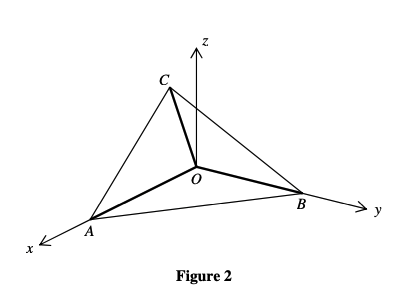
\includegraphics[width = .5\linewidth]{PPFigure2}
	\end{figure}
	\begin{enumerate}
		\item [(a)]
		\begin{enumerate}
			\item [(i)]Show that $$\overrightarrow{MN} = (a+b-1)\textbf{i} +(b-a) \textbf{j} +b \textbf{k}.$$
			\item [(ii)]Find the values of $a$ and $b$.
			\item [(iii)]Find the shortest distance between straight lines $AB$ and $OC$.
		\end{enumerate}
		(8 marks)
		\item [(b)]
		\begin{enumerate}
			\item [(i)]Find $\overrightarrow{AB}\times\overrightarrow{AC}$. 
			\item [(ii)]Let $G$ be the projection of $O$ on the plane $ABC$, find the coordinates of the intersecting point of the two straight lines $OG$ and $MN$.
		\end{enumerate}
		(5 marks)    
  	\end{enumerate}
	
	\newpage
	
	\item \textbf{HKDSE Math M2 2012 Q7}\\
	Figure 3 shows a parallelepiped $OADBECFG$. Let $\overrightarrow{OA} = 6\textbf{i} +2\textbf{j} -\textbf{k}$, $\overrightarrow{OB} = 2\textbf{i} +\textbf{j} $ and $\overrightarrow{OC} = 5\textbf{i} -\textbf{j} +2\textbf{k}$.
	\begin{figure}[H]
		\centering
		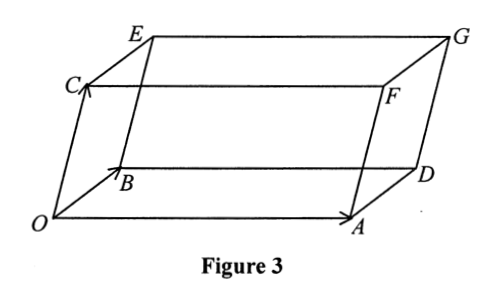
\includegraphics[width = .4\linewidth]{2012Figure3}
	\end{figure}
	\begin{enumerate}
		\item [(a)]Find the area of the parallelogram $OADB$. 
		\item [(b)]Find the distance between point $C$ and the plane $OADB$.
	\end{enumerate}
	(5 marks)

	\item \textbf{HKDSE Math M2 2012 Q12}\\
	Figure 6 shows an acute angled scalene triangle $ABC$, where $D$ is the mid-point of $AB$, $G$ is the centroid and $O$ is the circumcentre. Let $\overrightarrow{OA} = \textbf{a}$, $\overrightarrow{OB} = \textbf{b}$ and $\overrightarrow{OC} = \textbf{c}$.
	\begin{figure}[H]
		\centering
		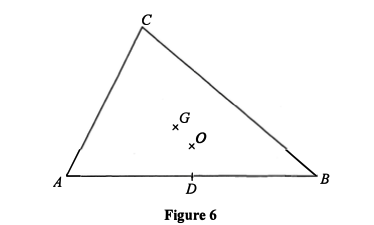
\includegraphics[width = .5\linewidth]{2012Figure6}
	\end{figure}
	\begin{enumerate}
		\item [(a)]Express $\overrightarrow{AG}$ in terms of $\textbf{a}$, $\textbf{b}$ and $\textbf{c}$.\\(3 marks)
		\item [(b)]It is given that $E$ is a point on $AB$ such that $CE$ is an altitude. Extend $OG$ to meet $CE$ at $F$. 
		\begin{enumerate}
			\item [(i)]Prove that $\triangle DOG \sim \triangle CFG$. \\
			Hence find $FG:GO$. 
			\item [(ii)]Show that $\overrightarrow{AF} = \textbf{b} + \textbf{c}$. \\
			Hence prove that $F$ is the orthocentre of $\triangle ABC$.
		\end{enumerate}
		(9 marks)
	\end{enumerate}
	
	\newpage
	
	\item \textbf{HKDSE Math M2 2013 Q10}\\
	Let $\overrightarrow{OA} = 2\textbf{i}$ and 
	$\overrightarrow{OB} = \textbf{i} +2 \textbf{j}$. $M$ is the mid-point of $OA$ and $N$ lies on $AB$ such that $BN : NA = k: 1$. $BM$ intersects $ON$ at $P$ (see Figure 2).
	\begin{figure}[H]
		\centering
		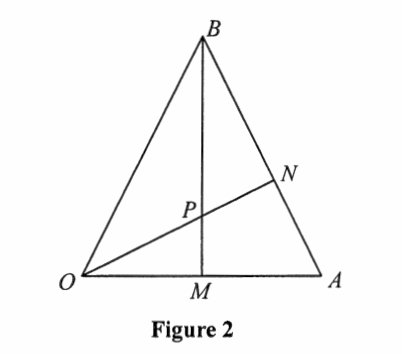
\includegraphics[width = .5\linewidth]{2013Figure2}
	\end{figure}
	\begin{enumerate}
		\item [(a)]Express $\overrightarrow{ON}$ in terms of $k$.
		\item [(b)]If $A$, $N$, $P$ and $M$ are concyclic, find the value of $k$.
	\end{enumerate}
	(5 marks)

	\item \textbf{HKDSE Math M2 2013 Q14}\\
	Figure 5 shows a fixed tetrahedron $OABC$ with $\angle AOB = \angle BOC = \angle COA = 90^{\circ}$. $P$ is a variable point such that $\overrightarrow{AP}\cdot\overrightarrow{BP} + \overrightarrow{BP}\cdot\overrightarrow{CP} + \overrightarrow{CP}\cdot\overrightarrow{AP} = 0$. Let $D$ be the fixed point such that $\overrightarrow{OD} = \displaystyle\frac{\overrightarrow{OA}+\overrightarrow{OB}+\overrightarrow{OC}}{3}$. \\
	Let $\overrightarrow{OA} = \textbf{a}$, $\overrightarrow{OB} = \textbf{b}$, $\overrightarrow{OC} = \textbf{c}$, $\overrightarrow{OP} = \textbf{p}$ and $\overrightarrow{OD} = \textbf{d}$. 
	\begin{figure}[H]
		\centering
		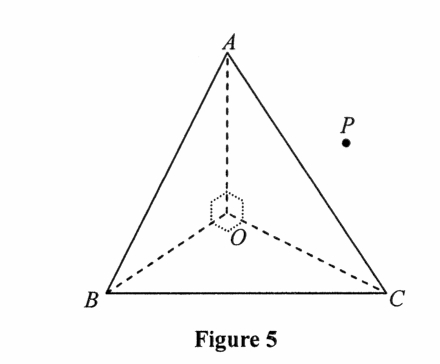
\includegraphics[width = .4\linewidth]{2013Figure5}
	\end{figure}
	\begin{enumerate}
		\item [(a)]
		\begin{enumerate}
			\item [(i)]Show that $\overrightarrow{AP}\cdot\overrightarrow{BP} = \textbf{p}\cdot\textbf{p} - (\textbf{a} + \textbf{b})\cdot\textbf{p}$. 
			\item [(ii)]Using (a)(i), show that $\textbf{p}\cdot\textbf{p} = 2\textbf{p}\cdot\textbf{d}$. 
			\item [(iii)]Show that $|\textbf{p} - \textbf{d}| = |\textbf{d}|$. \\
			Hence show that $P$ lies on the sphere centred at $D$ with fixed radius.
		\end{enumerate}
		(8 marks)
		\item [(b)]
		\begin{enumerate}
			\item [(i)]Alice claims that $O$ lies on the sphere mentioned in (a)(iii). Do you agree? Explain your answer. 
			\item [(ii)]Suppose $P_1$, $P_2$ and $P_3$ are three distinct points on the sphere in (a)(iii) such that $\overrightarrow{DP_1}\times\overrightarrow{DP_2} = \overrightarrow{DP_2}\times\overrightarrow{DP_3}$. Alice claims that the radius of the circle passing through $P_1$, $P_2$ and $P_3$ is $OD$. \\
			Do you agree? Explain your answer.
		\end{enumerate}
		(4 marks)
	\end{enumerate}

	\newpage

	\item \textbf{HKDSE Math M2 2014 Q8}\\
	Let 
	$\overrightarrow{OP} = -\textbf{i} +2 \textbf{j} +2\textbf {k}$, 
	$\overrightarrow{OQ} = \textbf{i} - \textbf{j} +2\textbf {k}$ and 
	$\overrightarrow{OR} = 2\textbf{i} -3 \textbf{j} +6\textbf {k}$. 
	\begin{enumerate}
		\item [(a)]Find $\overrightarrow{OP} \times \overrightarrow{OQ}$. \\
		Hence find the volume of tetrahedron $OPQR$. 
		\item [(b)]Find the acute angle between the plane $OPQ$ and the line $OR$, \\
		correct to the nearest $0.1^\circ$.
	\end{enumerate}
	(8 marks)

	\item \textbf{HKDSE Math M2 2014 Q11}\\
	In Figure 4, $C$ and $D$ are points on $OB$ and $OA$ respectively such that $AD : DO = OC : CB = t : 1-t$, where $0 < t < 1$. $BD$ and $AC$ intersect at $E$ such that $AE : EC = m : 1 $ and $BE : ED = n : 1 $, where $m$ and $n$ are positive. Let $\overrightarrow{OA} = \textbf{a}$ and $\overrightarrow{OB} = \textbf{b}$. 
	\begin{figure}[H]
		\centering
		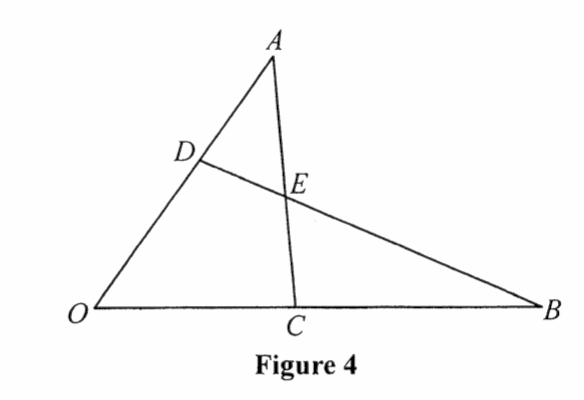
\includegraphics[width = .5\linewidth]{2014Figure4}
	\end{figure}
	\begin{enumerate}
		\item [(a)]
		\begin{enumerate}
			\item [(i)]By considering $\triangle OAC$, express $\overrightarrow{OE}$ in terms of $m$, $t$, $\textbf{a}$ and $\textbf{b}$.
			\item [(ii)]By considering $\triangle OBD$, express $\overrightarrow{OE}$ in terms of $n$, $t$, $\textbf{a}$ and $\textbf{b}$.
			\item [(iii)]Show that $\displaystyle m = \frac{t}{(1-t)^2}$ and $\displaystyle n = \frac{1-t}{t^2}$. 
			\item [(iv)]Chris claims that 
				$$\text{``if }m = n\text{, then }E\text{ is the centroid of }\triangle OAB\text{.''}$$
				Do you agree? Explain your answer.
		\end{enumerate}
		(9 marks)
		\item [(b)]It is given that $OA = 1$ and $OB = 2$. Francis claims that 
			$$``\text{if }AC\text{ is perpendicular to }OB\text{, then }BD\text{ is always perpendicular to }OA\text{.''}$$
			Do you agree? Explain your answer. \\(4 marks)
	\end{enumerate}

	\item \textbf{HKDSE Math M2 2015 Q10}\\
	$OAB$ is a triangle. $P$ is the mid-point of $OA$. $Q$ is a point lying on $AB$ such that $AQ : QB = 1 : 2$ while $R$ is a point lying on $OB$ such that $OR : RB = 3:1$. $PR$ and $OQ$ intersect at $C$. 
	\begin{enumerate}
		\item [(a)]		
		\begin{enumerate}
			\item [(i)]Let $t$ be a constant such that $PC : CR = t : (1-t)$.\\
				By expressing $\overrightarrow{OQ}$ in terms of $\overrightarrow{OA}$ and $\overrightarrow{OB}$, find the value of $t$. 
			\item [(ii)]Find $CQ:OQ$. 
		\end{enumerate}
		(7 marks)
		\item [(b)]Suppose that $\overrightarrow{OA} = 20\textbf{i} -6 \textbf{j} -12\textbf {k}$, $\overrightarrow{OB} = 16\textbf{i} -16 \textbf{j}$ and $\overrightarrow{OD} = \textbf{i} +3 \textbf{j} -6\textbf {k}$, where $O$ is the origin. Find
		\begin{enumerate}
			\item [(i)]the area of $\triangle OAB$, 
			\item [(ii)]the volume of tetrahedron $ABCD$.
		\end{enumerate}
		(5 marks)
	\end{enumerate}
	
	\newpage

	\item \textbf{HKDSE Math M2 2016 Q12}\\
	Let $\overrightarrow{OA} = 2 \textbf{j} +2\textbf {k}$, 
		$\overrightarrow{OB} = 4\textbf{i} + \textbf{j} + \textbf {k}$ and 
		$\overrightarrow{OP} = \textbf{i} +t \textbf{j}$, where $t$ is a constant and $O$ is the origin. It is given that $P$ is equidistant from $A$ and $B$. 
	\begin{enumerate}
		\item [(a)]Find $t$.\\(3 marks)
		\item [(b)]Let $\overrightarrow{OC} = 2 \textbf{i} - \textbf{j} +4\textbf {k}$ and $\overrightarrow{OD} = 3 \textbf{i} +2 \textbf{j} +5\textbf {k}$. Denote the plane which contains $A$, $B$ and $C$ by $\Pi$.
		\begin{enumerate}
			\item [(i)]Find a unit vector which is perpendicular to $\Pi$. 
			\item [(ii)]Find the angle between $CD$ and  $\Pi$. 
			\item [(iii)]It is given that $E$ is a point lying on $\Pi$ such that 
			$\overrightarrow{DE}$ is perpendicular to $\Pi$. Let $F$ be a point such that $\overrightarrow{PF} = \overrightarrow{PA} + \overrightarrow{PB} + \overrightarrow{PC}$. Describe the geometric relationship between $D$, $E$ and $F$. Explain your answer.
		\end{enumerate}
		(10 marks)
	\end{enumerate}

	\item \textbf{HKDSE Math M2 2017 Q3}\\
	$P$ is a point lying on $AB$ such that $AP : PB = 3:2$. Let $\overrightarrow{OA} = \textbf{a}$ and $\overrightarrow{OB} = \textbf{b}$, where $O$ is the origin.
	\begin{enumerate}
		\item [(a)] Express $\overrightarrow{OP} $ in therms of $ \textbf{a}$ and $ \textbf{b}$.
		\item [(b)] It is given that $|\textbf{a}| = 45$, $|\textbf{b}| = 20$ and $\cos{\angle{AOB}} = \displaystyle\frac{1}{4}$. Find
		\begin{enumerate}
			\item [(i)] $\textbf{a}   \cdot  \textbf{b} $, 
			\item [(ii)] $|\overrightarrow{OP}| $. 
		\end{enumerate}
	\end{enumerate}
	(5 marks)

	\item \textbf{HKDSE Math M2 2017 Q10}\\
	$ABC$ is a triangle. $D$ is the mid-point of $AC$. $E$ is a point lying on $BC$ such that $BE : EC = 1 : r$. \\
	$AB$ produced and $DE$ produced meet at the point $F$. It is given that $DE : EF = 1 : 10$. \\
	Let $\overrightarrow{OA} = 2\textbf{i} +3 \textbf{j} -2\textbf {k}$, 
		$\overrightarrow{OB} = 4\textbf{i} +4 \textbf{j} - \textbf {k}$, 
		$\overrightarrow{OC} = 8\textbf{i} -3 \textbf{j} -2\textbf {k}$, where $O$ is the origin.
	\begin{enumerate}
		\item [(a)]By expressing $\overrightarrow{AE}$ and $\overrightarrow{AF}$ in terms of $r$, find $r$.\\(4 marks)
		\item [(b)]
		\begin{enumerate}
			\item [(i)]Find $\overrightarrow{AD} \cdot \overrightarrow{DE}$. 
			\item [(ii)]Are $B, D, C$ and $F$ concyclic? Explain your answer.
		\end{enumerate}
		(5 marks)
		\item[(c)]Let $\overrightarrow{OP} = 3\textbf{i} +10 \textbf{j} -4\textbf {k}$. Denote the circumcentre of $\triangle BCF $ by $ Q$.\\
		Find the volume of the tetrahedron $ABPQ$.\\(3 marks)
	\end{enumerate}

	\item \textbf{HKDSE Math M2 2018 Q12}\\
	The position vectors of the points $A, B, C$ and $D$ are  
	$4\textbf{i} -3 \textbf{j} + \textbf {k}$, 
	$-\textbf{i} +3 \textbf{j} -3 \textbf {k}$, 
	$7\textbf{i} - \textbf{j} +5 \textbf {k}$ and 
	$3\textbf{i} -2 \textbf{j} -5 \textbf {k}$  
	respectively. Denote the plane which contains $A, B$ and $C$ by $\Pi$. Let E be the projection of  $D$ on $\Pi$.
	\begin{enumerate}
		\item [(a)]Find
		\begin{enumerate}
			\item [(i)]$\overrightarrow{AB} \times \overrightarrow{AC}$,
			\item [(ii)]the volume of the tetrahedron $ABCD$,
			\item [(iii)]$\overrightarrow{DE}$.
		\end{enumerate}
		(5 marks)
		\item [(b)]Let $F$ be a point lying on $BC$ such that $DF$ is perpendicular to $BC$.
		\begin{enumerate}
			\item [(i)]Find $\overrightarrow{DF}$. 
			\item [(ii)]Is $\overrightarrow{BC} $ perpendicular to $\overrightarrow{EF}$ ? Explain your answer.
		\end{enumerate}
		(5 marks)
		\item[(c)]Find the angle between $\triangle BCD$ and $\Pi$. \\(3 marks)
	\end{enumerate}
	
	\newpage

	\item \textbf{HKDSE Math M2 2019 Q12}\\
	Let $\overrightarrow{OA} = \textbf{i} -4 \textbf{j}+ 2\textbf {k}$, $\overrightarrow{OB} = -5\textbf{i} -4 \textbf{j} +8\textbf {k}$ and $\overrightarrow{OC} = -5\textbf{i} -12 \textbf{j} +t\textbf {k}$, where $O$ is the origin and $t$ is a constant. It is given that $|\overrightarrow{AC}| = |\overrightarrow{BC}|$. 
	\begin{enumerate}
		\item [(a)]Find $t$. \\(3 marks)
		\item [(b)]Find $\overrightarrow{AB} \times \overrightarrow{AC}$. \\(2 marks)
		\item [(c)]Find the volume of the pyramid $OABC$. \\(2 marks)
		\item [(d)]Denote the plane which contains $A$, $B$ and $C$ by $\Pi$. It is given that $P$, $Q$ and $R$ are points lying on $\Pi$ such that $\overrightarrow{OP} = p\textbf{i}$, $\overrightarrow{OQ} = q\textbf{j}$ and $\overrightarrow{OQ} = r\textbf{k}$. Let $D$ be the projection of $O$ on $\Pi$.
		\begin{enumerate}
			\item [(i)]Prove that $pqr \neq 0$. 
			\item [(ii)]Find $\overrightarrow{OD}$. 
			\item [(ii)]Let $E$ be a point such that $\overrightarrow{OE} = \displaystyle\frac{1}{p}\textbf{i}+\frac{1}{q}\textbf{j}+\frac{1}{r}\textbf{k}$. Describe the geometric relationship between $D$, $E$ and $O$. Explain your answer.
		\end{enumerate}
		(6 marks)
	\end{enumerate}

	\item \textbf{HKDSE Math M2 2020 Q12}\\
	Let $\overrightarrow{OP} = \textbf{i} + \textbf{j}+ 4\textbf {k}$ and $\overrightarrow{OQ} = 5\textbf{i} -7 \textbf{j}- 4\textbf {k}$, where $O$ is the origin. \\
	$R$ is a point lying on $PQ$ such that $PR:RQ = 1:3$. 
	\begin{enumerate}
		\item [(a)]Find $\overrightarrow{OP} \times \overrightarrow{OR}$. \\(2 marks)
		\item [(b)]Define $\overrightarrow{OS} = \overrightarrow{OP} + \overrightarrow{OR}$. Find the area of the quadrilateral $OPSR$. \\(2 marks)
		\item [(c)]Let $N$ be a point such that $\overrightarrow{ON} = \lambda(\overrightarrow{OP}\times \overrightarrow{OR})$, where $\lambda$ is a real number.
		\begin{enumerate}
			\item [(i)]Is $\overrightarrow{NR}$ perpendicular to $\overrightarrow{PQ}$? Explain your answer.
			\item [(ii)]Let $\mu$ be a real number such that $\overrightarrow{NQ}$ is parallel to $11\textbf{i} + \mu\textbf{j}-10\textbf {k}$. 
			\begin{enumerate}
				\item [(1)]Find $\lambda$ and $\mu$. 
				\item [(2)]Denote the angle between $\triangle OPQ$ and $\triangle NPQ$ by $\theta$. Find $\tan{\theta}$.
			\end{enumerate}
		\end{enumerate}
		(8 marks)
	\end{enumerate}

	\item \textbf{HKDSE Math M2 2021 Q12}\\
	The position vectors of the points $A$, $B$, $C$ and $D$ are  $t\textbf{i} +14 \textbf{j}+s \textbf {k}$, $12\textbf{i} -s \textbf{j}-2 \textbf {k}$, $(s+2)\textbf{i} -16 \textbf{j}+10 \textbf {k}$ and $-t\textbf{i} +(s+2) \textbf{j}+14 \textbf {k}$  respectively, where $s$, $t \in \mathbb{R}$. Suppose that $\overrightarrow{AB}$ is parallel to $5\textbf{i} -4 \textbf{j}-2 \textbf {k}$. \\Denote the plane which contains $A$, $B$ and $C$ by $\Pi$.
	\begin{enumerate}
		\item [(a)]Find
		\begin{enumerate}
			\item [(i)]$s$ and $t$,
			\item [(ii)]the area of $\triangle ABC$,
			\item [(iii)]the volume of the tetrahedron $ABCD$,
			\item [(iv)]the shortest distance from $D$ to $\Pi$.
		\end{enumerate}
		(9 marks)
		\item [(b)]Let $E$ be the projection of  $D$ on $\Pi$. Is $E$ the circumcentre of $\triangle ABC$? Explain your answer.\\(4 marks)
	\end{enumerate}
	
	\newpage

	\item \textbf{HKDSE Math M2 2022 Q12}\\
	Consider $\triangle ABC$. Denote the origin by $O$. 
	\begin{enumerate}
		\item [(a)]Let $D$ be a point lying on $BC$ such that $AD$ is the angle bisector of $\angle BAC$. \\
		Define $BC = a$, $AC = b$  and  $AB = c$. 
		\begin{enumerate}
			\item [(i)]Using the fact that $BD:DC = c:b$, prove that $$\overrightarrow{AD} = -\overrightarrow{OA}+\displaystyle\frac{b}{b+c}\overrightarrow{OB} + \displaystyle\frac{c}{b+c}\overrightarrow{OC}.$$
			\item [(ii)]Let $E$ be a point lying on $AC$ such that $BE$ is the angle bisector of $\angle ABC$. \\
			Define $$\overrightarrow{OJ} = \displaystyle\frac{a}{a+b+c}\overrightarrow{OA}+\displaystyle\frac{b}{a+b+c}\overrightarrow{OB}+\displaystyle\frac{c}{a+b+c}\overrightarrow{OC}.$$
				Prove that $J$ lies on $AD$. Hence, deduce that $AD$ and $BE$ intersect at $J$.
		\end{enumerate}
		(7 marks)
		\item [(b)]Suppose that $\overrightarrow{OA} = 35\textbf{i} +9 \textbf{j}+ \textbf {k}$, $\overrightarrow{OB} = 40\textbf{i} -3 \textbf{j}+ \textbf {k}$ and $\overrightarrow{OC} =  -3 \textbf{j}+ \textbf {k}$. Let $I$ be the incentre of $\triangle ABC$. 
		\begin{enumerate}
			\item [(i)] Find $\overrightarrow{OI}$. 
			\item [(ii)] By considering $\overrightarrow{AI} \times \overrightarrow{AB}$, find the radius of the inscribed circle of $\triangle ABC$. 
		\end{enumerate}
		(5 marks)
	\end{enumerate}            

	\item \textbf{HKDSE Math M2 2023 Q10}\\
	Let $O$ be the origin. The position vectors of $P$ and $Q$ are $-2\textbf{i} - \textbf{k}$ and $2\textbf{i} -\textbf{j}+ \textbf{k}$ respectively. Denote the circle passing through $O$, $P$ and $Q$ by $C$. Let $R$ be a point lying on $PQ$ such that $OR$ is perpendicular to $OQ$.
	\begin{enumerate}
		\item [(a)] By considering the ratio of $PR$ to $RQ$, find $\overrightarrow{OR}$. \\(3 marks)
		\item [(b)] $OR$ produced meets $C$ at another point $S$. Find $\overrightarrow{OS}$. \\(3 marks)
		\item [(c)] Let $\Pi$ be the plane which contains $C$.
		\begin{enumerate}
			\item [(i)] Find a non-zero vector which is perpendicular to $\Pi$.
			\item [(ii)] Let $G$ be the center of $C$. Denote the projection of point $A(-6, -22,2)$ on $\Pi$ by $B$. Describe the geometric relationship between $O$, $B$ and $G$. Explain your answer.
		\end{enumerate}
		(6 marks)
	\end{enumerate}

\end{enumerate}
\end{document}